\chapter{Results}\label{chap:results}

In this chapter an overview over the different evaluations and exploration tools created in this work is given. To acquire results, a short description of the processing is provided in section \ref{sec:results}. The section \ref{subsec:result_tables} shows several result tables and describes how to read and interpret the specific values.  As a few examples of evaluating the \glspl{kpi}, in section \ref{sec:visuals} a collection of visualization can be seen.
\section{Result Evaluation}\label{sec:results}
To evaluate the data set a collection of processing was done using the sql alchemy package, similar to the insert mechanism of the measurement values in the consumer paragraph of section \ref{subsec:software}. Additionally normalized tables, containing standardized 15 min intervals were created (refer to the 'Sensor\_Meta\_tables') to visualize a longer time amount in the visualization tool (refer to section \ref{subsec:RPMT}). Due to hardware and connection difficulties, data of sensor 32 did not suffice for evaluation, and has been omitted in all tables. The values of the tables in section \ref{subsec:result_tables} allow comparison of total consumption measurements, minima, maxima and averages, which were processed using SQL queries. The values are calculated similar to the equations \ref{eq:min}, \ref{eq:max} and \ref{eq:avg} respectively. 
\begin{equation}\label{eq:min}
	MIN (X) = x_i \bigg\rvert x_i, x_j \in X \wedge \not \exists x_j \geq x_i \wedge i < j
\end{equation}

\begin{equation}\label{eq:max}
	MAX (X) = x_i \bigg\rvert x_i, x_j \in X \wedge \neg \exists x_j \geq x_i \wedge i < j
\end{equation}

\begin{equation}\label{eq:avg}
	AVG (X) = \dfrac{\sum_{i=1}^{n}{x_i}}{n} \bigg\arrowvert x_i \in X \wedge |X| = n 
\end{equation}
To enable quick reference, the section \ref{subsec:insights} collects key observations gathered from the results, and shows relations that were expected by related works.
\subsection{Quantitative Results}\label{subsec:result_tables}
As a reference, the average consumption values of user 1 per day, can be seen in table \ref{tab:user1}. Date values range from 1st of June to 29th of Juli, where only weekdays are considered. The respective average values give information on the consumption rate of the specific day, while the ratio of the averages show a difference in energy conservation during off work hours. The evaluation shows two levels of days with no work activity. These days are recognizable by consumption values around 0.6 to 1.4 watts of average consumption, and virtually no difference between weekday - and workday average. The small difference between the 0.6 Watt values (e.g. 12th to 15th of Juli) and the 1.4 Watt values (e.g. 6th and 7th of June) could be explained due to for example a single device in standby (e.g. the monitor). Most activity days show good \acrshort{wwcr} values around 2, with single outliers like 21st, 22nd and 25th of Juli, that lack any consumption reduction during off hours. On the whole the average of user 1 fits the expectations of a user that is predominantly conscious of energy efficiency, while showing signs of inconsistency.\\
\begin{table}
	\centering
	\begin{tabular}{|l|c|c|}
		Date& weekday average (W)& workday average (W)\\
		2022-06-01&     7.1246&     6.3368\\
		2022-06-02&   62.9861&    86.5046\\
		2022-06-03&  66.9280 &   88.5383\\
		2022-06-06 &  1.3643 &    1.3644\\
		2022-06-07&   1.3649 &    1.3698\\
		2022-06-08&  41.0420 &   82.9115
		\\ 2022-06-09 & 23.3274 &   47.8767
		\\ 2022-06-10  & 1.3873 &    1.3913
		\\ 2022-06-13  &27.9845 &   58.8300
		\\ 2022-06-14  &25.1870 &   54.9713
		\\ 2022-06-15  &26.6638 &   42.9791
		\\ 2022-06-16  & 1.4900 &    1.4924
		\\ 2022-06-17  & 1.1917 &    1.1950
		\\ 2022-06-20  &27.2710 &   52.8197
		\\ 2022-06-21  & 0.6530 &    0.6566
		\\ 2022-06-22  &24.2942 &   46.9040
		\\ 2022-06-23   &1.1986 &    1.1995
		\\ 2022-06-24   &1.1978 &    1.1989
		\\ 2022-06-27   &1.1941 &    1.1971
		\\ 2022-06-28   &1.1968 &    1.1994
		\\ 2022-06-29   &1.1948 &    1.1964
		\\ 2022-06-30  &26.1305 &   53.3058
		\\ 2022-07-01  &1.1950   &  1.1951
		\\ 2022-07-04  &25.0155  &  50.5588
		\\ 2022-07-05   &0.6521 &    0.6518
		\\ 2022-07-06  &16.1277&    30.7782
		\\ 2022-07-07   &0.6357&     0.6368
		\\ 2022-07-08   &0.6367&    0.6365
		\\ 2022-07-11  &18.3418&  42.5024
		\\ 2022-07-12   &0.6354&    0.6352
		\\ 2022-07-13   &0.6340&     0.6345
		\\ 2022-07-14   &0.6331&     0.6321
		\\ 2022-07-15   &0.6328&     0.6344
		\\ 2022-07-18  &21.9215&    44.9616
		\\ 2022-07-19  &20.3028&    41.4121
		\\ 2022-07-20  &34.3390&    51.1681
		\\ 2022-07-21  &43.7019&    43.7787
		\\ 2022-07-22  &43.7082&    43.7739
		\\ 2022-07-25  &22.2650&    16.1565
		\\ 2022-07-26  &25.6874&    54.4252
		\\ 2022-07-27  &22.0577&    45.2281
		\\ 2022-07-28  &28.0511&    53.5048
		\\ 2022-07-29   &1.0874&     1.0907
	\end{tabular}
	\caption{Consumption results of user 1 in Watts.}
	\label{tab:user1}
\end{table}
The tables \ref{tab:sensor} and \ref{tab:sensor_cont} show the number of available measurement days, their average values and \acrfull{wwcr}. The tables give an individual insight into specific average weekday consumption, which is useful to estimate electricity demands of similar devices. As the number of days approach the 55 days duration of the evaluation range, the resulting values increase in accuracy. The addition of workday averages is then used to compute the \acrshort{wwcr} of each device respectively. This ratio can be used as an indicator to differentiate users and devices that actively reduce consumption outside of work hours. It can be clearly seen that unused sensor outlets possess a \acrshort{wwcr} of about $1$ while values from around 1.3 show little active consumption reduction during off hours. On the other extreme values around 2.3 show a great change of consumption during off hours, which either shows extremely high consumption which would be indicated by a very high \gls{workday} value, or a great reduction which is mostly indicated here.\\
The evaluation of different workplaces gain little insight as max consumption spike way higher in Mutli devices, which indicates, that workplaces are not really comparable to each other, as consumption differs greatly. Furthermore the higher amount of false 'negative' consumption in the unused working spaces further distort the consumption data elements in the data set. As almost all the \acrshortpl{wwcr} of negative sensor averages approximate 1, the odd values can be attributed to bias of the sensor, as noise should impact the averages slightly differently. The surprising value of 0.4 \acrshort{wwcr} returned on sensor 16 can be seen as a product of noise due to the low numeric values in the milliwatts range. Positive average measurements contain low frequency occupation of workplaces like sensor 28 and 29 due to low averages.\\
\begin{table}[h]
	\centering
	\begin{tabular}{l|c|c|c|c}
		Sensor Number & \# of days & weekday avg (W) & workday avg (W)& workday to weekday ratio \\
		1 & 55 & 5.3293 & 8.8202 & 1.6550 \\
		2 & 12 & 8.0936 & 13.6496 & 1.6865 \\ 
		3 & 55 & 5.8806 & 9.5379 & 1.6219  \\ 
		4 & 55 & 2.0053 & 4.0004 & 1.9948 \\
		5 & 55 & 1.9414 & 4.0445 & 2.0833 \\
		6 & 54 & 2.8747 & 5.8710 & 2.0423 \\ 
		7 & 51 & 5.8539 & 10.1643 & 1.7363  \\ 
		8 & 55 & 3.5986 & 7.9214 & 2.2012 \\
		9 & 55 & 3.6589 & 8.1175 & 2.2186 \\
		10 & 55 & 1.4391 & 3.0190 & 2.098 \\
		11 & 55 & 2.2525 & 4.6371 & 2.0586 \\ 
		12 & 55 & 0.1333 & 0.1426 & 1.0690 \\
		13 & 55 & 6.7418 & 10.2663 & 1.5228 \\
		14 & 55 & 0.3329 & 0.4553 & 1.3676 \\
		15 & 55 & 0.0672 & 0.1052 & 1.5660 \\
		16 & 55 & -0.0668 & -0.0333 & 0.4980 \\
		17 & 55 & 1.6774 & 3.5020 & 2.0877 \\
		18 & 55 & 2.2333 & 4.6420 & 2.0786 \\
		19 & 55 & -0.1789 & -0.1780 & 0.9948 \\
		20 & 55 & -0.0805 & -0.0804 & 0.9990 \\ 
		21 & 55 & -0.0880 & -0.0878 & 0.9987 \\
		22 & 55 & 17.3964 & 18.2880 & 1.0512 \\
		23 & 55 & 6.8836 & 14.1276 & 2.0523 \\
		24 & 55 & 2.3189 & 4.8253 & 2.0809 \\
	\end{tabular}
	\caption{Result table of average \gls{workday}, and weekday consumption of sensor 1 to 24 in Watts. Continuation follows in table \ref{tab:sensor_cont}.}
	\label{tab:sensor}
\end{table}
\begin{table}[h]
	\centering
	\begin{tabular}{l|c|c|c|c}
		Sensor Number & \# of days & weekday avg & workday avg & workday to weekday ratio \\
		25 & 55 & 3.5589 & 7.4198 & 2.0848 \\
		26 & 55 & 3.4856 & 6.9230 & 1.9862 \\
		27 & 55 & 0.1361 & 0.1875 & 1.3776 \\
		28 & 55 & 0.5605 & 1.2871 & 2.2964 \\
		29 & 55 & 2.2456 & 4.4983 & 2.0032 \\
		30 & 55 & 17.6872 & 27.9409 & 1.5797 \\
		31 & 55 & -0.1473 & -0.1462 & 0.9922 \\
		33 & 55 & 10.4353 & 20.2452 & 1.9401 \\
		34 & 55 & 4.7989 & 8.5369 & 1.7789 \\
		35 & 55 & 0.7072 & 0.8253 & 1.1670 \\
		36 & 55 & 27.0940 & 36.2963 & 1.3396 \\
		37 & 55 & 45.8122 & 65.0602 & 1.4201 \\
	\end{tabular}
	\caption{Result table of average \gls{workday}, and weekday consumption of sensor 25 to 37 in Watts. Precursory available in result table \ref{tab:sensor}.}
	\label{tab:sensor_cont}
\end{table}
To examine differences in workplace organization, tables \ref{tab:multi_wp}, \ref{tab:dual_workplace} and \ref{tab:singleworkplace} show overview values of the respective workplace type. Each table shows the corresponding Devices, their overall minimum and maximum consumption value on record, as well as the average consumption across the evaluation period. Each final row shows a 'Total' value that represents the total minimum, maximum and average of the values of the table above. This final row in each table shows the peak consumption value in them, and the respective device can be determined, and the average total consumption can again be used to estimate consumption of similar workplaces. Dual workplace evaluations contain a large number of vacant or changing occupation during the measurement period. Due to this a relevant comparison between the workplaces gives little insight in their comparison. As indicated by the maximum values, the resulting consumption should be expected to be comparable, a final evaluation does not provide this kind of conclusion. As total values of dual workplaces should be in similar ranges, the fact that averages differ beyond factor 2 cannot be easily ignored. This leads to the theory that workload and/or occupation frequency is very different between the workplaces, and the individual consumption of the users do not scale linearly in dual workplaces irrespective of the type of work and work frequency (like part time to full time employment or home office times).\\The workplace evaluation, completed by the results in table \ref{tab:singleworkplace} gives little insights when comparing absolute values. The issue is, that due to no information on the comparability of each workload in a given workplace, the reduction or increase in consumption can be explained from energy efficiency, to time efficiency with high work consumption, to normal time efficiency averaging a low work consumption.
\begin{table}[h]
	\centering
		\begin{tabular}{l|c|c|c|c}
		\multicolumn{5}{c}{Workplace 3} \\
		Device ID & Device Type & min power (W)& max power (W)& avg consumption (W)\\
		14 & PC & -0.3 & 276.4 & 2.0851 \\
		15 & Monitor & -0.3 & 15.2 & 0.7428 \\
		16 & PC & -0.2 & 42.7 & -0.0822 \\
		17 & Monitor & -0.4 & 13.2 & 0.8994 \\
		18 & Monitor & -0.3 & 17.5 & 1.1453 \\
		19 & PC & -0.3 & 15.8 & -0.1230 \\
		20 & Monitor & -0.2 & 44.6 & -0.0705 \\
		21 & Monitor & -0.2 & 0.0 & -0.0885 \\
		22 & Printer & -0.2 & 2671.0 & 16.4998 \\
		\hline
		Total & Multiple & -0.4 & 2671.0 & 21.0078
	\end{tabular}
	\begin{tabular}{l|c|c|c|c}
		\multicolumn{5}{c}{Workplace 4} \\
		Device ID & Device Type & min power (W)& max power (W)& avg consumption (W)\\
		23 & PC &-0.1 & 89.8 & 2.7413 \\
		24 & Monitor & -0.3 & 15.3 & 0.8937 \\
		25 & Monitor & -0.4 & 21.3 & 1.3511 \\
		26 & PC & -0.8 & 208.7 & 3.6216 \\
		27 & Monitor & -0.2 & 26.7 & 0.9517 \\
		28 & Monitor & -0.3 & 22.3 & 0.9721 \\
		29 & Monitor & -0.3 & 22.3 & 1.6204 \\
		30 & PC & -2.8 & 2152.8 & 10.2244 \\
		31 & Monitor & -0.3 & 0.0 & -0.1449 \\
		\hline
		Total & Multiple & -2.8 & 2152.8 & 22.2318
	\end{tabular} 
	\begin{tabular}{l|c|c|c|c}
		\multicolumn{5}{c}{Workplace 5} \\
		ID & Type & min power (W)& max power (W)& avg consumption (W)\\
		33 & PC & 0.3 & 243.2 & 8.2019 \\
		\hline
		Total& Multiple & 0.3 & 243.2 & 8.2019 \\
	\end{tabular}
	\caption{Result table of Workplaces of type multiple (more than 2 potential users).}
	\label{tab:multi_wp}
\end{table}
\begin{table}[h]
	\centering
	\begin{tabular}{l|c|c|c|c}
		\multicolumn{5}{c}{Workplace 1} \\
		ID & Type & min power (W)& max power (W)& avg consumption (W)\\
		4 & PC & -0.2 & 20.6 & 1.0352 \\
		5 & Monitor & -0.2 & 21.1 & 0.7207 \\
		6 & Monitor & -0.2 & 70.2 & 1.7565 \\
		7 & PC & -0.3 & 114.7 & 6.2446 \\
		8 & Monitor & -0.3 & 35.9 & 4.1898 \\
		9 & Monitor & -0.2 & 33.4 & 3.5638 \\
		\hline
		Total & Multiple & -0.3 & 114.7 o& 17.5104
	\end{tabular}
	\begin{tabular}{l|c|c|c|c}
		\multicolumn{5}{c}{Workplace 6} \\
		ID & Type & min power (W)& max power (W)& avg consumption (W)\\
		34 & Multiple & -0.3 & 127.9 & 6.1979 \\
		35 & Multiple & -0.4 & 105.8 & 0.5758 \\
		\hline
		Total & Multiple & -0.4 & 127.9 & 6.7738
	\end{tabular}
	\begin{tabular}{l|c|c|c|c}
		\multicolumn{5}{c}{Workplace 7} \\
		ID & Type & min power (W)& max power (W)& avg consumption (W)\\
		36 & Multiple & 10.3 & 1180.5 & 27.7893 \\
		37 & Multiple & 0.7 & 257.4 & 43.2404 \\
		\hline
		Total & Multiple & 0.7 & 1180.5 & 72.0296
	\end{tabular}
	\caption{Result table of workplaces of type Dual (exactly 2 potential users).}
	\label{tab:dual_workplace}
\end{table}
\begin{table}[h]
	\begin{tabular}{l|c|c|c|c}
		\multicolumn{5}{c}{Workplace 0} \\
		ID & Type & min power (W)& max power (W)& avg consumption (W)\\
		1 & PC & -0.2 & 91.2 & 5.8942 \\
		2 & Monitor & -0.2 & 33.3 & 5.1298 \\
		3 & Monitor & -0.1 & 33.5 & 6.6894 \\
		\hline
		Total & Multiple & -0.2 & 91.2 & 17.7135
	\end{tabular}
	\begin{tabular}{l|c|c|c|c}
		\multicolumn{5}{c}{Workplace 2} \\
		ID & Type & min power (W)& max power (W)& avg consumption (W)\\
		10 & PC & -0.2 & 18.4 & 1.1847 \\
		11 & Monitor & -0.2 & 83.4 & 1.6731 \\
		12 & Printer & -0.6 & 289.8 & 0.1327 \\
		13 & Utility & -0.2 & 2523.0 & 4.8885 \\
		\hline 
		Total & Multiple & -0.6 & 2523.0 & 7,8792
	\end{tabular}
	\caption{Result table of workplaces of type single (exactly one potential user).}
	\label{tab:singleworkplace}
\end{table}
In tables \ref{tab:PCMon} and \ref{tab:devices} a direct comparison of the individual types of devices can be made. Each table consists of the collection of devices of matching type, showing all time minimum, maximum and average consumption measurements. The respective total row of each tabular can be used to determine the consumption ratio of each type of device to the total consumption. In this instance, the multiple type broadly consist of a mixture of all other device types and is ignored in the type differentiation. Interestingly the sum of all recorded single devices almost exactly equals the total consumption of all Multi device sensors (sum of 86.34 to Multi measurement 86.01). The resulting mix of consumption computes to 38\% PC, 37\% Monitors, 6\% Utilities and 19\% through Printing. The average measured consumption adds up to 172.35 Watts and an hourly CO$_2$ footprint of 61.3 g of direct emission through electricity consumption. This gives a yearly footprint estimation of at least 0.38 tons of CO$_2$ using 260 working days a year and assuming zero emissions on the remaining days. By estimations of atmosfair, this equates to about a quarter of the estimated allowed CO$_2$ budget of a person until 2050, to remain in alignment with the Paris agreement \cite{co2_capita}. 
\begin{table}[h]
	\centering
	\begin{tabular}{l|c|c|c}
		\multicolumn{4}{c}{Device type PC} \\
		ID & min power (W)& max power (W)& avg consumption (W)\\
		1 & -0.2 & 91.2 & 5.8942\\
		4 & -0.2 & 20.6 & 1.0352 \\
		7 & -0.3 & 114.7 & 6.2446 \\
		10 & -0.2 & 18.4 & 1.1847 \\
		14 & -0.3 & 276.4 & 2.0851 \\
		16 & -0.2 & 42.7 & -0.0822 \\
		19 & -0.3 & 15.8 & -0.1230 \\
		23 & -0.1 & 89.8 & 2.7412 \\
		26 & -0.8 & 208.7 & 3.6216 \\
		30 & -2.8 & 2152.8 & 10.2244 \\
		\hline
		Total & -2.8 & 2152.8 & 32.8260 \\
	\end{tabular}
	
	\begin{tabular}{l|c|c|c}
		\multicolumn{4}{c}{Device type Monitor} \\
		ID & min power (W)& max power (W)& avg consumption (W)\\
		2 & -0.2 & 33.3 & 5.1298 \\
		3 & -0.1 & 33.5 & 6.6894 \\
		5 & -0.2 & 21.1 & 0.7207 \\
		6 & -0.2 & 70.2 & 1.7565 \\
		8 & -0.3 & 35.9 & 4.1898 \\
		9 & -0.2 & 33.4 & 3.5638 \\
		11 & -0.2 & 83.4 & 1.6731 \\
		15 & -0.3 & 15.2 & 0.7428 \\
		17 & -0.4 & 13.2 & 0.8993 \\
		18 & -0.3 & 17.5 & 1.1453 \\
		20 & -0.2 & 44.6 & -0.0705 \\
		21 & -0.2 & 0.0 & -0.0885 \\
		24 & -0.3 & 15.3 & 0.8937 \\
		25 & -0.4 & 21.3 & 1.3511 \\
		27 & -0.2 & 26.7 & 0.9517 \\
		28 & -0.3 & 22.3 & 0.9721 \\
		29 & -0.3 & 22.3 & 1.6204 \\
		31 & -0.3 & 0.0 & -0.1449 \\
		\hline
		Total & -0.4 & 83.4 &31.995 \\
	\end{tabular}
	\caption{Result table showing average consumption of PC and Monitor devices.}
	\label{tab:PCMon}
\end{table}
\begin{table}[h]
	\centering
	\begin{tabular}{l|c|c|c}
		\multicolumn{4}{c}{Device type Utility} \\
		ID & min power (W)& max power (W)& avg consumption (W)\\
		13 & -0.2 & 2523 & 4.8885 \\
	\end{tabular}
	\begin{tabular}{l|c|c|c}
		\multicolumn{4}{c}{Device type Printer} \\
		ID & min power (W)& max power (W)& avg consumption (W)\\
		12 & -0.6 & 289.8 & 0.1327 \\
		22 & -0.2 & 2671.0 & 16.4998 \\
		\hline
		Total & -0.6 & 2671.0 & 16.6324
	\end{tabular}
	\begin{tabular}{l|c|c|c}
		\multicolumn{4}{c}{Device type Multiple} \\
		ID & min power (W)& max power (W)& avg consumption (W)\\
		34 & -0.3 & 127.9 & 6.1979 \\
		37 & 0.7 & 257.4 & 43.2403 \\
		36 & 10.3 & 1180.5 & 27.7893 \\
		33 & 0.3 & 243.2 & 8.2019 \\
		35 & -0.4 & 105.8 & 0.5758 \\
		\hline
		Total & -0.4 & 1180.5 &86.0055 \\ 
	\end{tabular}
	\caption{Result table showing average consumption of Utility, Printer and Multi devices.}
	\label{tab:devices}
\end{table}

\paragraph{Idle Time} as defined in equation \ref{eq:idle} was calculated using the meta\_tables of each device, wherever available. The results can be seen in tabular \ref{tab:idle} consisting of the device, the corresponding workplace, and the resulting idle time in absolute and relative terms. While working as intended with Computer and Monitoring devices, which indicate reasonable working hours of the devices of averaging to about 4 hours of usage per workday. This should be a reasonable estimate considering 7 hour workdays dispersed with home office and holiday vacancies. Devices with higher off hour consumption like the type of printer used monitored by sensor 22 show no idle time at all, which would indicate usage without interruption. This observation does not hold when comparing consumption profiles using heat maps, as seen in section \ref{sec:visuals}.
\begin{table}[ht]
	\centering
	\begin{tabular}{|l|c|c|c|c|c|}%
		\hline%
		Sensor&Device&Workplace&Workplace Type&Idle Time&Idle Time in \%\\%
		\hline%
		Sensor 1&PC&0&Single&4909&84 \%\\%
		\hline%
		Sensor 2&Monitor&0&Single&3786&83 \%\\%
		\hline%
		Sensor 3&Monitor&0&Single&4919&84 \%\\%
		\hline%
		Sensor 4&PC&1&Dual&5023&87 \%\\%
		\hline%
		Sensor 5&Monitor&1&Dual&5116&87 \%\\%
		\hline%
		Sensor 6&Monitor&1&Dual&4546&84 \%\\%
		\hline%
		Sensor 7&PC&1&Dual&0&0 \%\\%
		\hline%
		Sensor 8&Monitor&1&Dual&4974&85 \%\\%
		\hline%
		Sensor 9&Monitor&1&Dual&4992&85 \%\\%
		\hline%
		Sensor 10&PC&2&Single&5412&92 \%\\%
		\hline%
		Sensor 11&Monitor&2&Single&5405&92 \%\\%
		\hline%
		Sensor 12&Printer&2&Single&5845&100 \%\\%
		\hline%
		Sensor 13&Utility&2&Single&0&0 \%\\%
		\hline%
		Sensor 14&PC&3&Single&5612&96 \%\\%
		\hline%
		Sensor 15&Monitor&3&Single&5706&97 \%\\%
		\hline%
		Sensor 16&PC&3&Single&5842&100 \%\\%
		\hline%
		Sensor 17&Monitor&3&Single&4908&84 \%\\%
		\hline%
		Sensor 18&Monitor&3&Single&4904&84 \%\\%
		\hline%
		Sensor 19&PC&3&Single&5856&100 \%\\%
		\hline%
		Sensor 20&Monitor&3&Single&5843&100 \%\\%
		\hline%
		Sensor 21&Monitor&3&Single&5856&100 \%\\%
		\hline%
		Sensor 22&Printer&3&Single&0&00 \%\\%
		\hline%
		Sensor 23&PC&4&Multi&4990&85 \%\\%
		\hline%
		Sensor 24&Monitor&4&Multi&5094&87 \%\\%
		\hline%
		Sensor 25&Monitor&4&Multi&5094&87 \%\\%
		\hline%
		Sensor 26&PC&4&Multi&5059&86 \%\\%
		\hline%
		Sensor 27&Monitor&4&Multi&5848&100 \%\\%
		\hline%
		Sensor 28&Monitor&4&Multi&5826&99 \%\\%
		\hline%
		Sensor 29&Monitor&4&Multi&5039&86 \%\\%
		\hline%
		Sensor 30&PC&4&Multi&5019&86 \%\\%
		\hline%
		Sensor 31&Monitor&4&Multi&5856&100 \%\\%
		\hline%
		Sensor 33&Multiple&5&Multi&0&0 \%\\%
		\hline%
		Sensor 34&Multiple&6&Dual&4309&74 \%\\%
		\hline%
		Sensor 35&Multiple&6&Dual&5762& 98 \%\\%
		\hline%
		Sensor 36&Multiple&7&Dual&0&0 \%\\%
		\hline%
		Sensor 37&Multiple&7&Dual&0&0 \%\\%
		\hline%
	\end{tabular}
	\caption{Overview of the calculated idle times of each device. The Idle Time column shows the number of intervals (15 minutes) with a power reading of less than 1 Watt.}
	\label{tab:idle}
\end{table} 

\subsection{Key Insights}\label{subsec:insights}
\noindent The device type evaluation gives parts of the expected results from the literature\cite{min-energy}, that consumption due to monitoring is very comparable to processing consumption as seen in the average consumption values of table \ref{tab:PCMon}. Apparently the different advances in energy efficiency in screens and computer performance seem to balance nicely, as literature values are more than 10 years obsolete. The difference of a few percentage points in consumption (38\% to 44\% for Monitoring, 37\% to 39\%) do not indicate huge progression differences. From another perspective, IT workers should be sensitized to the fact that dual monitor setups increase consumption by roughly 33\% compared to single monitor setups.\\
Evaluations in workplace contexts show no clear relations regarding energy consumption. Real work frequency(full time, part time or remote work), and classification of work for each user are likely the major contributor to determine total energy consumption than the individual workplace structure. This evaluation can change if the usage profile of the experiment is not representative of a usual working environment.\\
\acrfull{wwcr} delivers a suitable measure to differentiate users of similar consumption averages. This can be used to determine possible saving methodologies to increase the ratio by consumption reduction during off work hours on individuals that could harbor a greater saving potential.\\
Idle time is unsuitable for device agnostic measurements, and needs to be modified according to the expected usage profile of a specific device and the bias / noise effects on the used sensors.

\section{Visualizations}\label{sec:visuals}
Time series data is in many ways well suited to visualized. However,
to accommodate for differences in timestamp usage, all database tables created for visualization should use epoch time in milliseconds. This format is used in the sensor\_meta tables, to ease their usage in Grafana. However, different tools can require another format to visualize the time series, and the conversions can be made accordingly using simple division constants. While different applications define epoch base up to the nanoseconds, this kind of application does not benefit from higher frequencies, as HTTP requests provide a lower temporal resolution. 

\subsubsection{Heat maps}
To visualize an overview of consumption over time, in this section a collection of comparable plots are displayed. In figure \ref{fig:user_comparison} the accumulated data for each distinct user can be seen in a row, with whole day values on the left, and data limited to \gls{workday} hours on the right. A great difference in coloring between the left and right sides indicate a high \gls{wwcr} for this user. If devices between users are comparable this indicates either a high consumption during work hours or an effort of energy saving after and before work hours. This evaluation shows to be less effective with short consumption peaks, like in barely used workplaces (see fig \ref{fig:user_comparison} row 5 and 12 for reference).
As expected, differences between users regarding their \gls{wwcr} can be seen, as well as the less frequented working spaces due to their color extremes. User 14 shows little difference between \gls{workday} and weekday values, which indicates little change of energy consumption during off hours, which means a greater potential of energy efficiency gain should be expected by reducing off hour consumption. As a counter example user 10 can be examined, which shows a bigger color change and narrower distribution. Generally a drop in consumption on Fridays can be examined.  With this kind of analysis, a more directed package of intervention mechanism can be explored, to improve performance of less dedicated users with higher reduction potential. The Indication of the quantitative analysis of user 1 given in the section \ref{subsec:result_tables} using table \ref{tab:user1} can be confirmed using the heat map, as color changes can be clearly seen in comparison of the depictions in the first row. Further of interest is the visualization of user 7 which shows high consumption on weekends. This is the result of constant negative measurements due to noise and a slight sensor bias, as weekend values were not considered, which results in a 0 value in visualization. This fact especially has to be considered when handling measurements including real "negative" measurements due to localized power generation.\\
Figure \ref{fig:office_consumption} shows the summation of all power consumption on weekdays. Additionally the heat maps were generated using only specific device types. The different kinds of devices that were considered are PCs (see figure \ref{fig:pc_hm}), Monitors (see figure \ref{fig:mon_hm}), Printer (see figure \ref{fig:printer_hm}) and Utilities (see figure \ref{fig:util_hm}). As expected, the color scheme of PC consumption coincides very well with monitor usage, but not very well with printer usage. This indicates external factors to the printer usage besides attendance for example (i.e. exams or meetings/out of office gatherings). These kinds of illustrations can be useful to determine patterns in cooperation, that quantitative information does not allow. \hskip
\begin{figure}[ht]
    \centering
    \subfloat{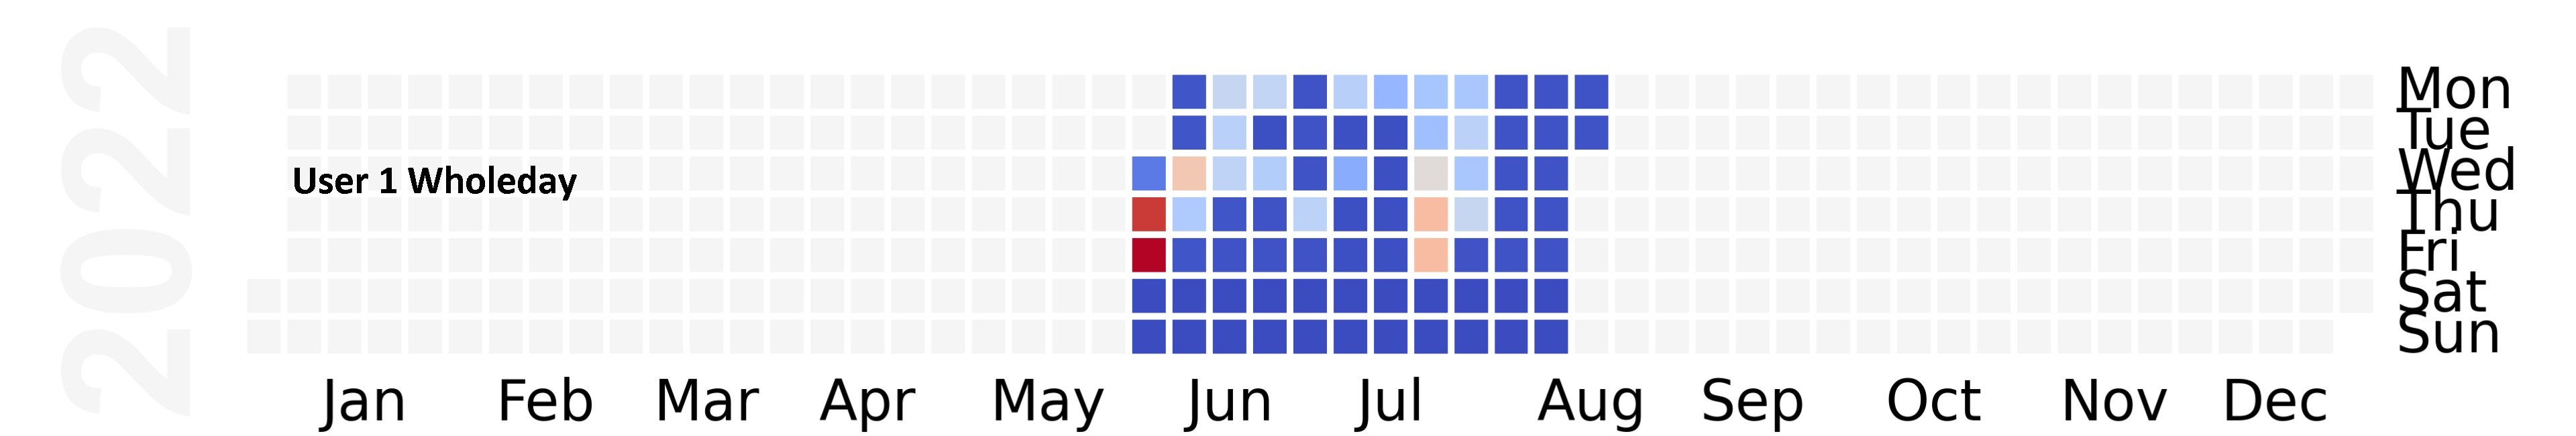
\includegraphics[width=0.5\textwidth]{images/heatmaps/user_1_wholeday_cal.png}}
    \subfloat{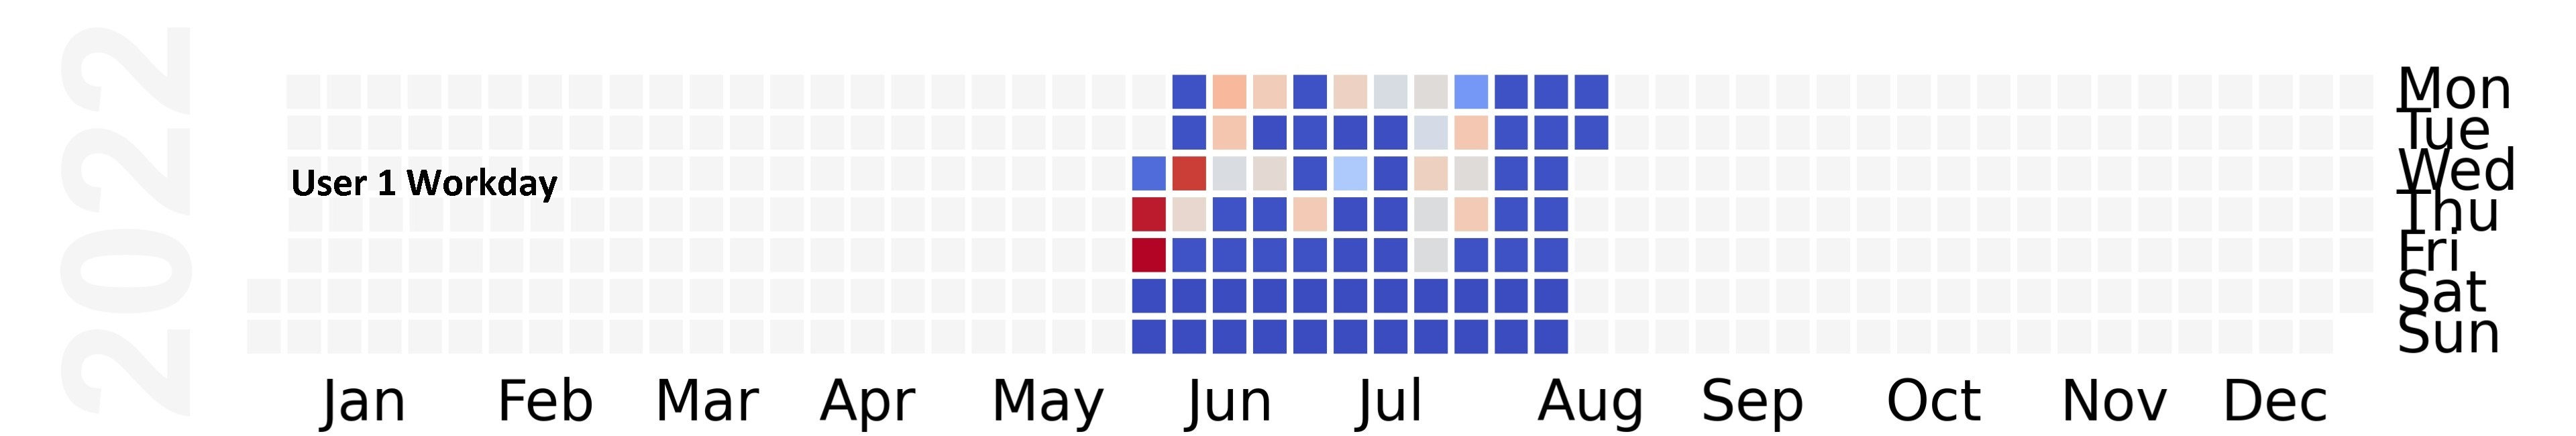
\includegraphics[width=0.5\textwidth]{images/heatmaps/user_1_workday_cal.png}}\newline
    \subfloat{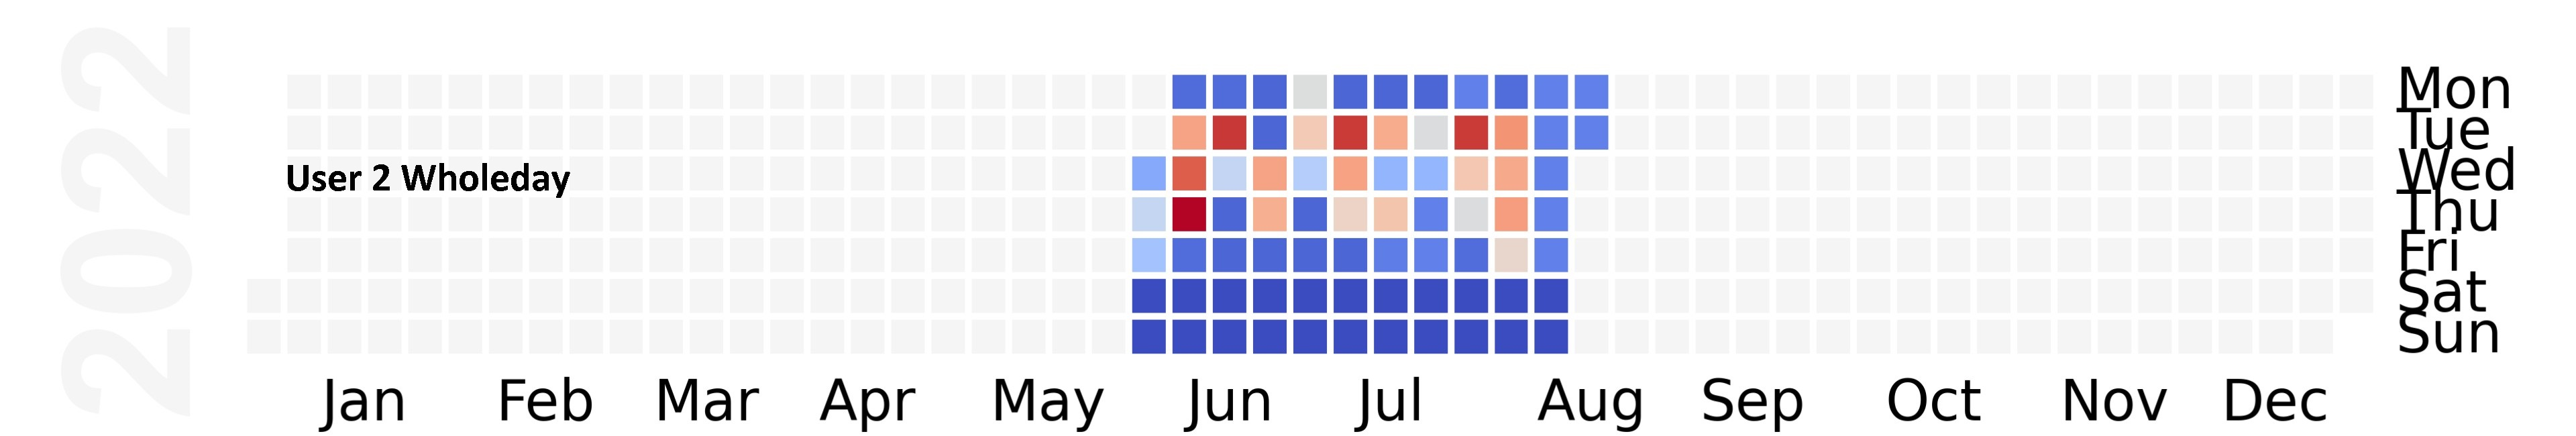
\includegraphics[width=0.5\textwidth]{images/heatmaps/user_2_wholeday_cal.png}}
    \subfloat{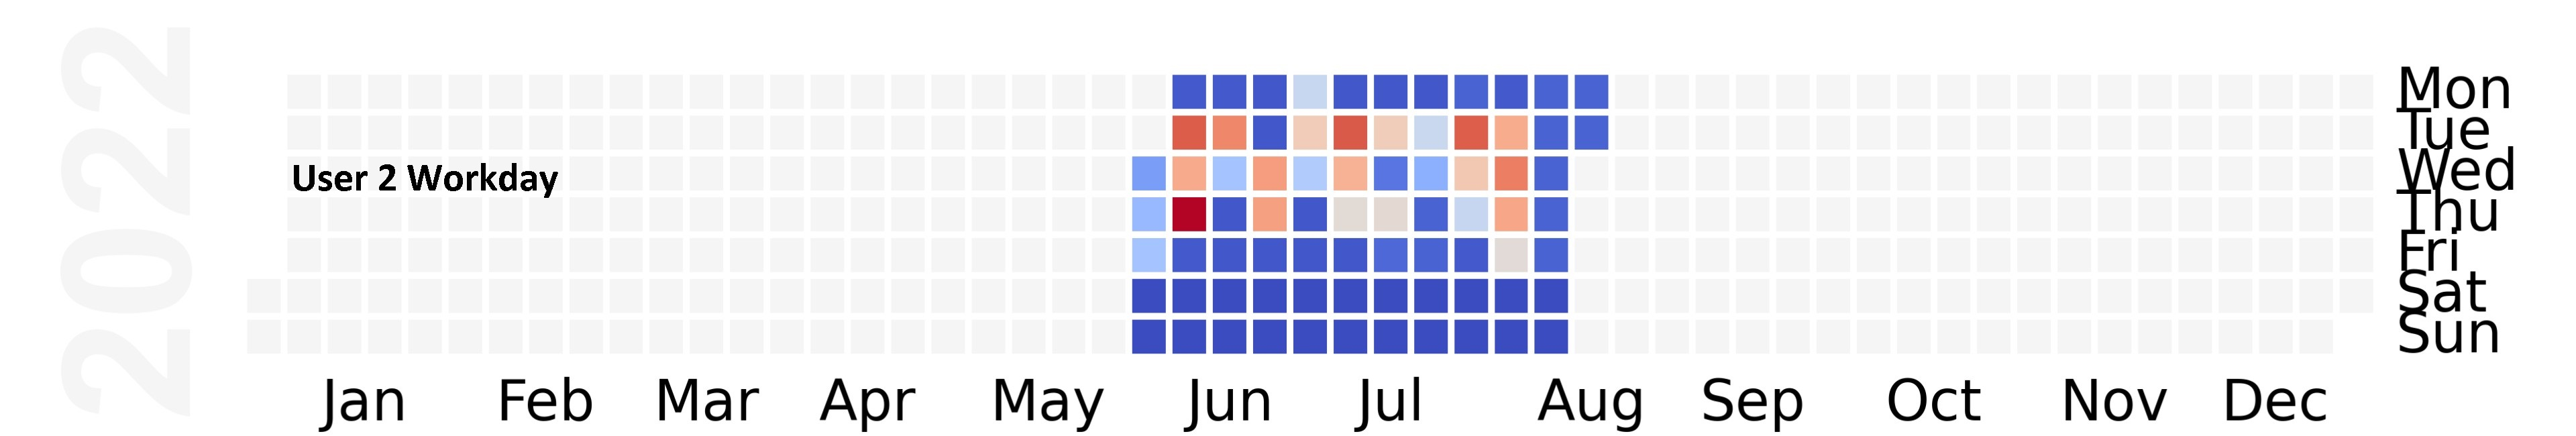
\includegraphics[width=0.5\textwidth]{images/heatmaps/user_2_workday_cal.png}}\newline
    \subfloat{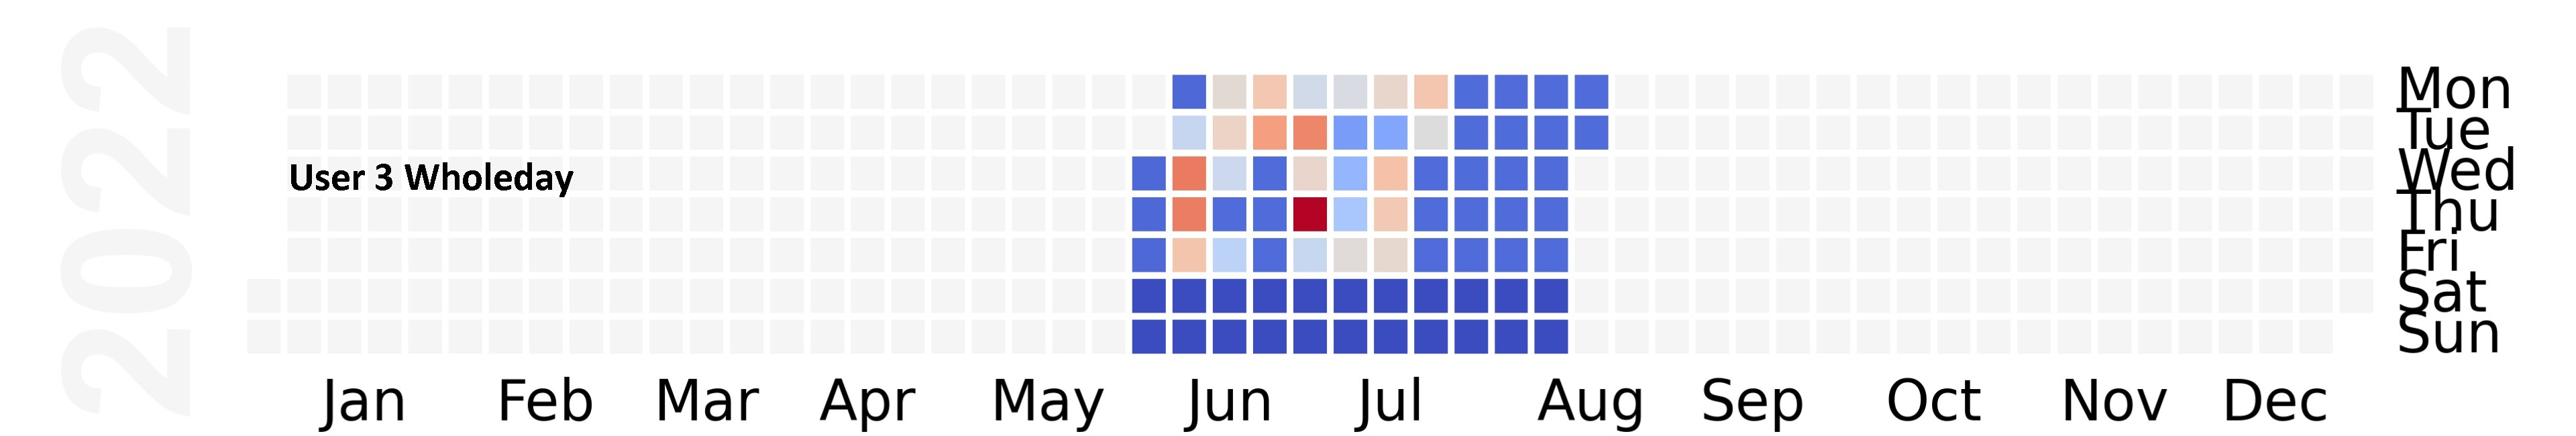
\includegraphics[width=0.5\textwidth]{images/heatmaps/user_3_wholeday_cal.png}}
    \subfloat{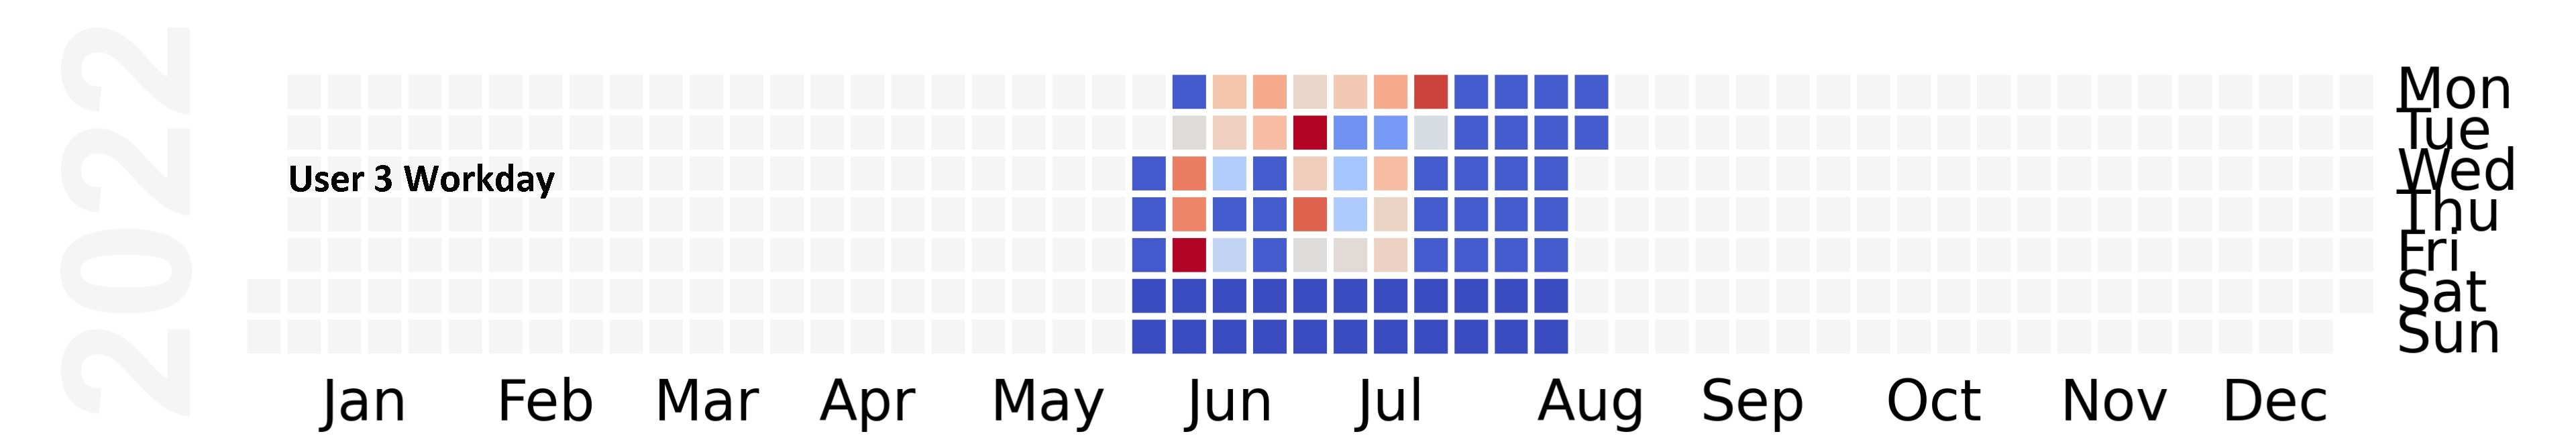
\includegraphics[width=0.5\textwidth]{images/heatmaps/user_3_workday_cal.png}}\newline
    \subfloat{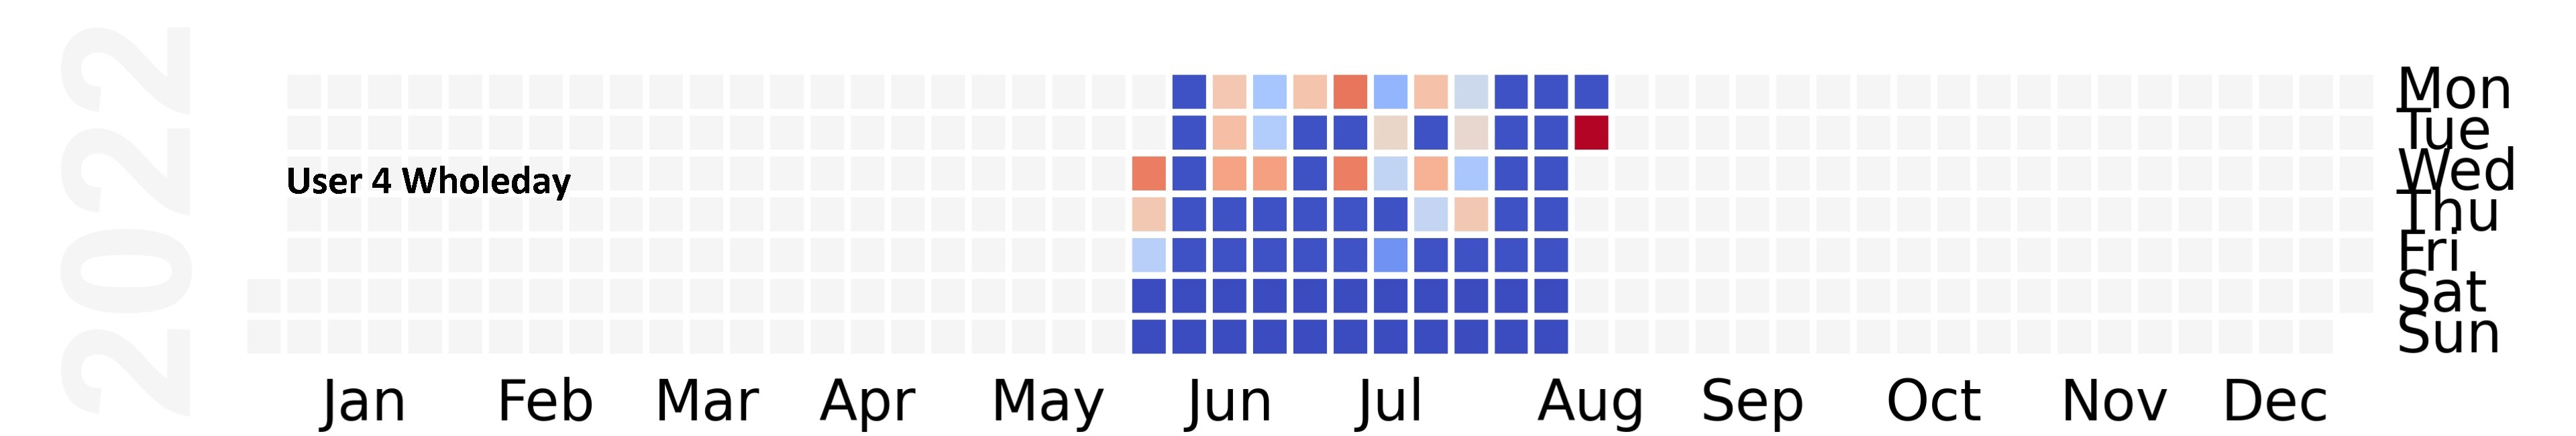
\includegraphics[width=0.5\textwidth]{images/heatmaps/user_4_wholeday_cal.png}}
    \subfloat{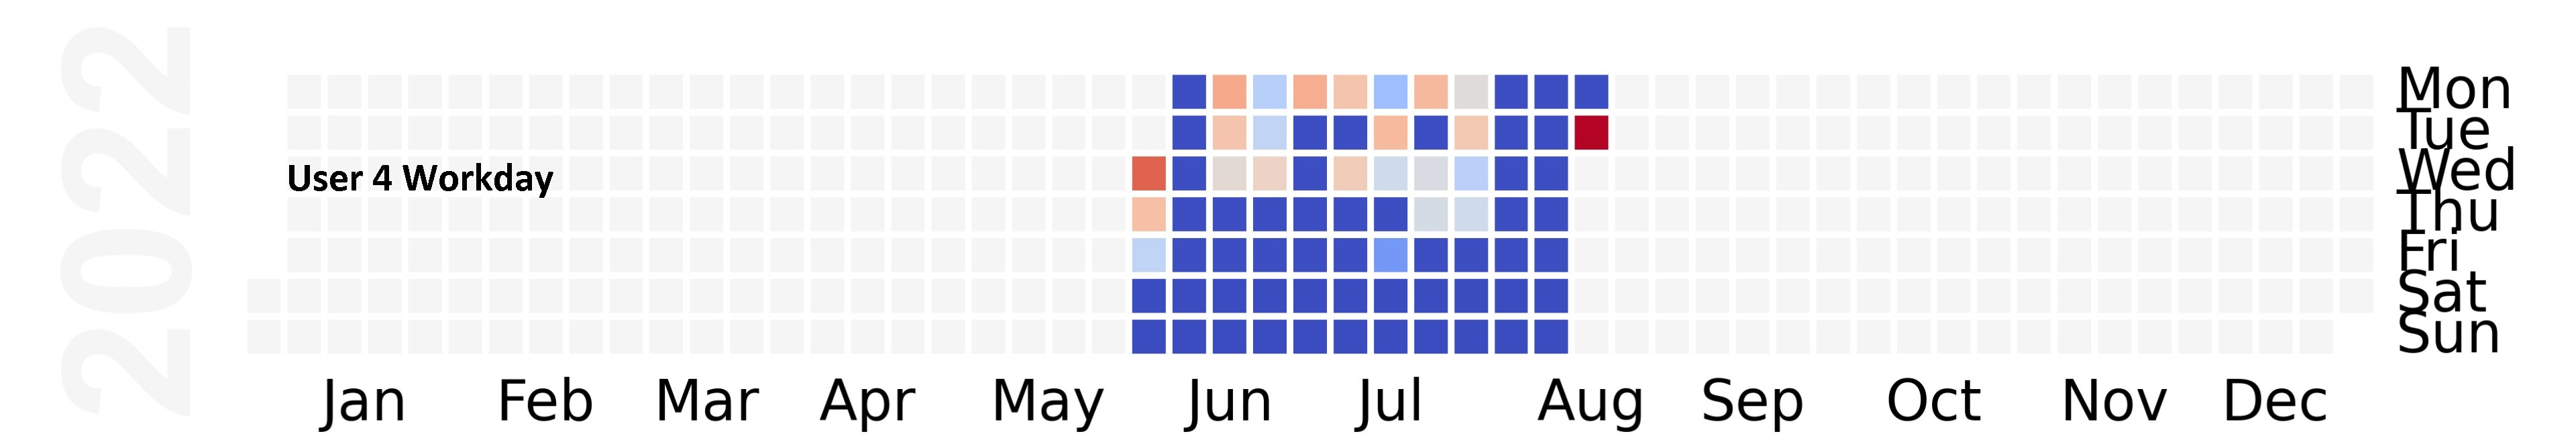
\includegraphics[width=0.5\textwidth]{images/heatmaps/user_4_workday_cal.png}}\newline
    \subfloat{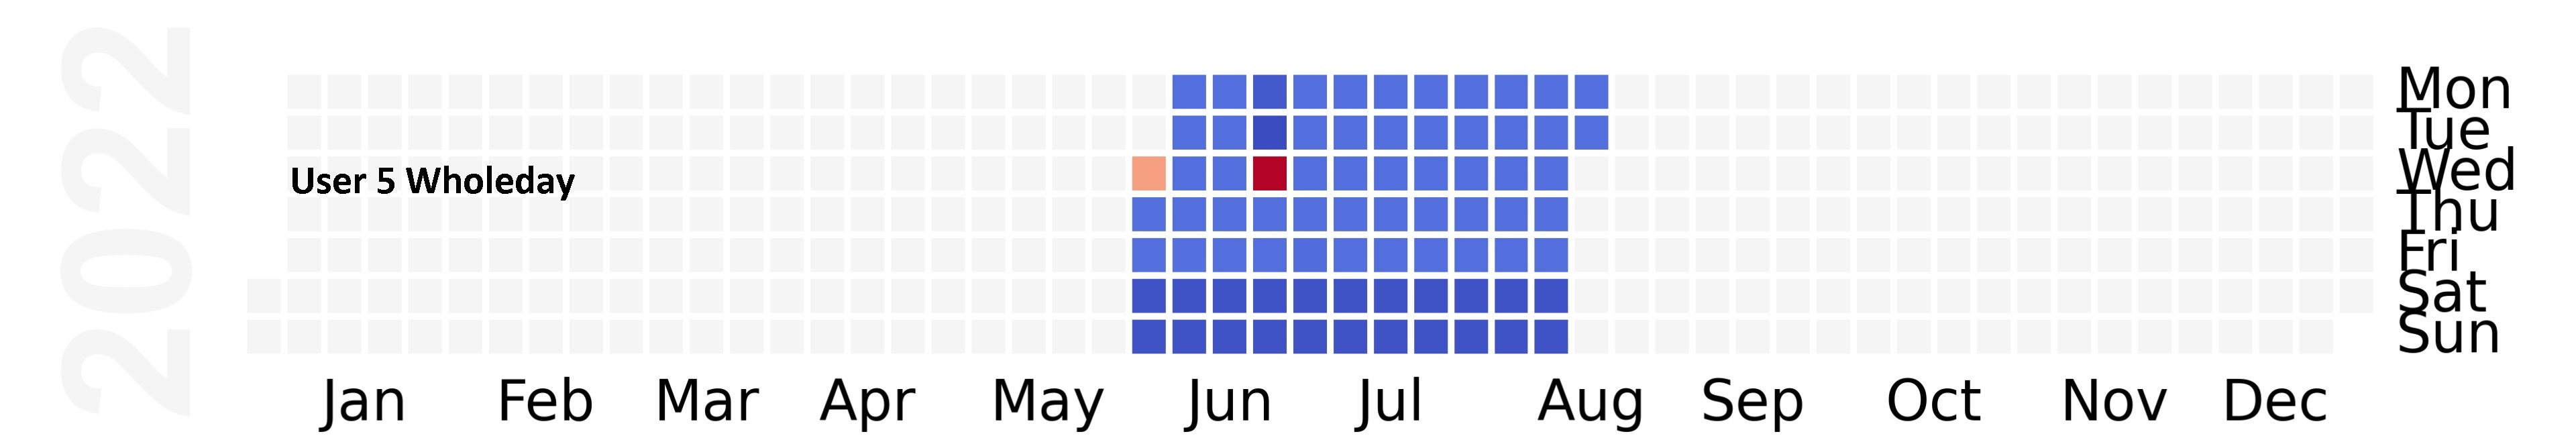
\includegraphics[width=0.5\textwidth]{images/heatmaps/user_5_wholeday_cal.png}}
    \subfloat{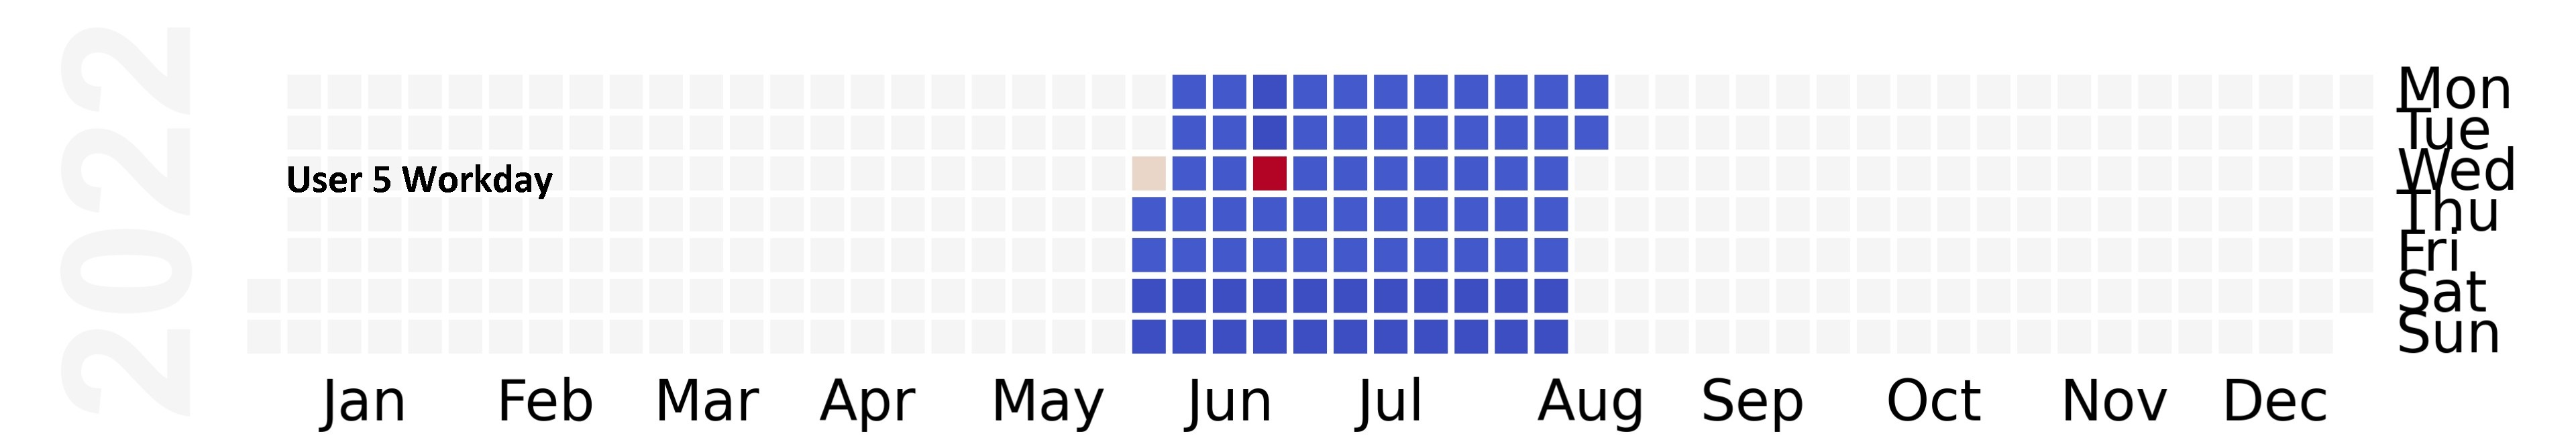
\includegraphics[width=0.5\textwidth]{images/heatmaps/user_5_workday_cal.png}}\newline
    \subfloat{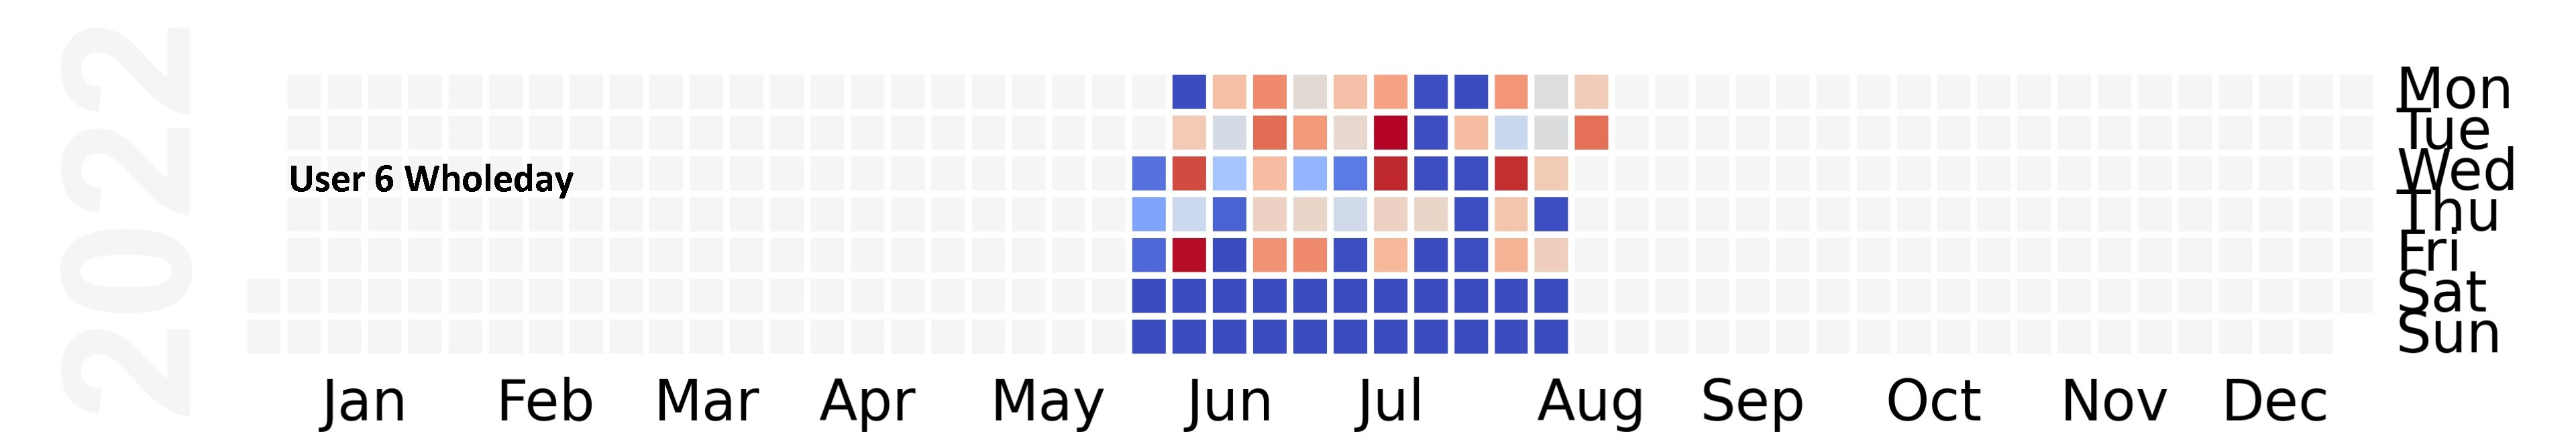
\includegraphics[width=0.5\textwidth]{images/heatmaps/user_6_wholeday_cal.png}}
    \subfloat{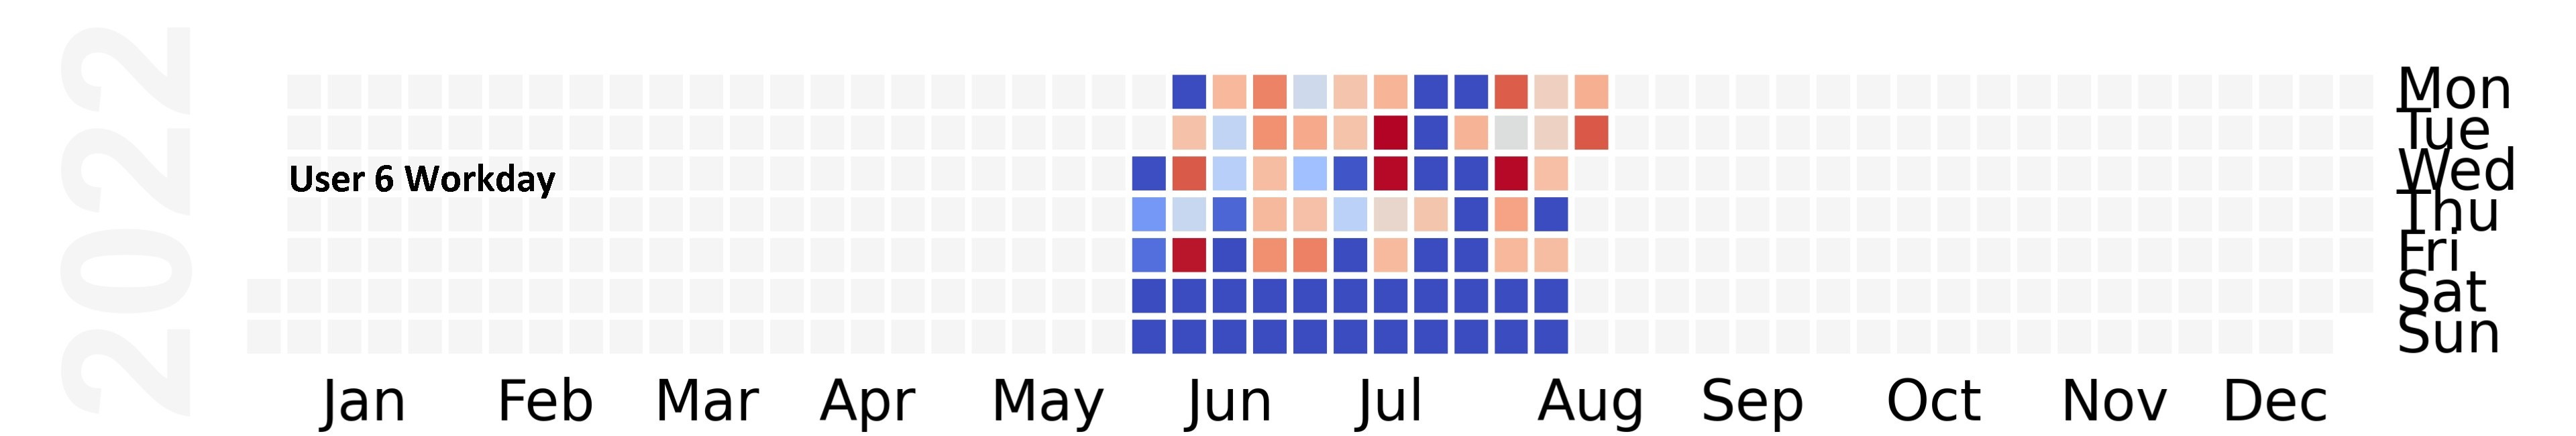
\includegraphics[width=0.5\textwidth]{images/heatmaps/user_6_workday_cal.png}}\newline
        \subfloat{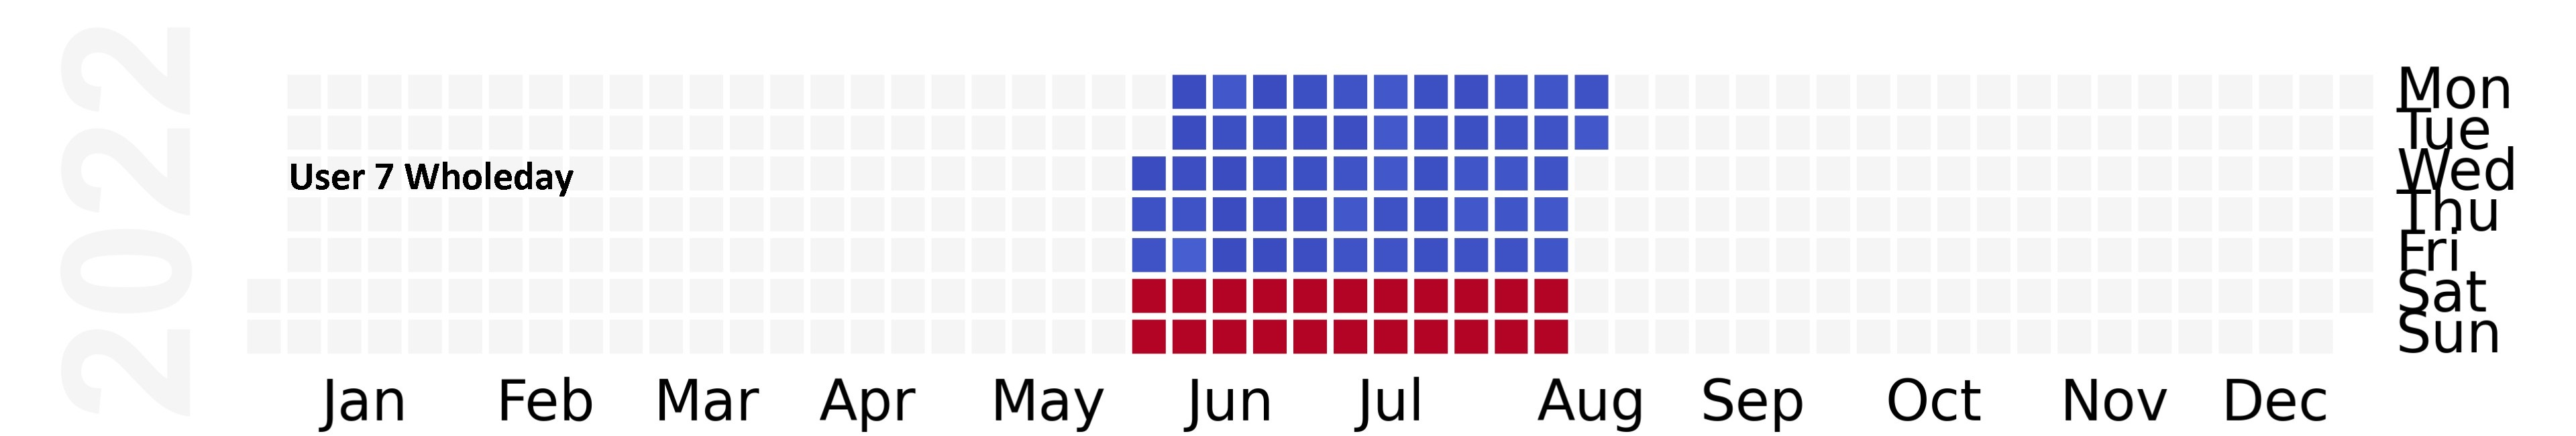
\includegraphics[width=0.5\textwidth]{images/heatmaps/user_7_wholeday_cal.png}}
    \subfloat{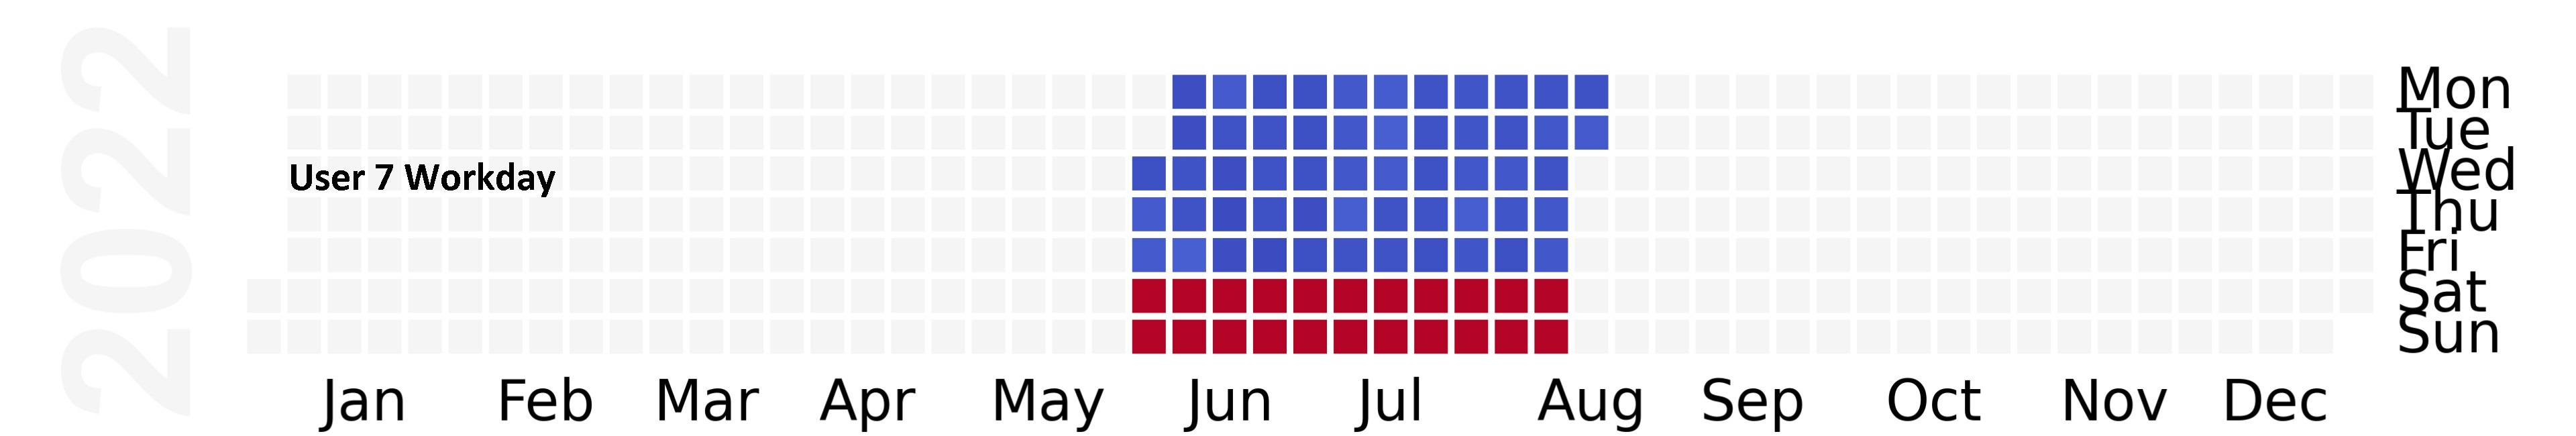
\includegraphics[width=0.5\textwidth]{images/heatmaps/user_7_workday_cal.png}}\newline
    \subfloat{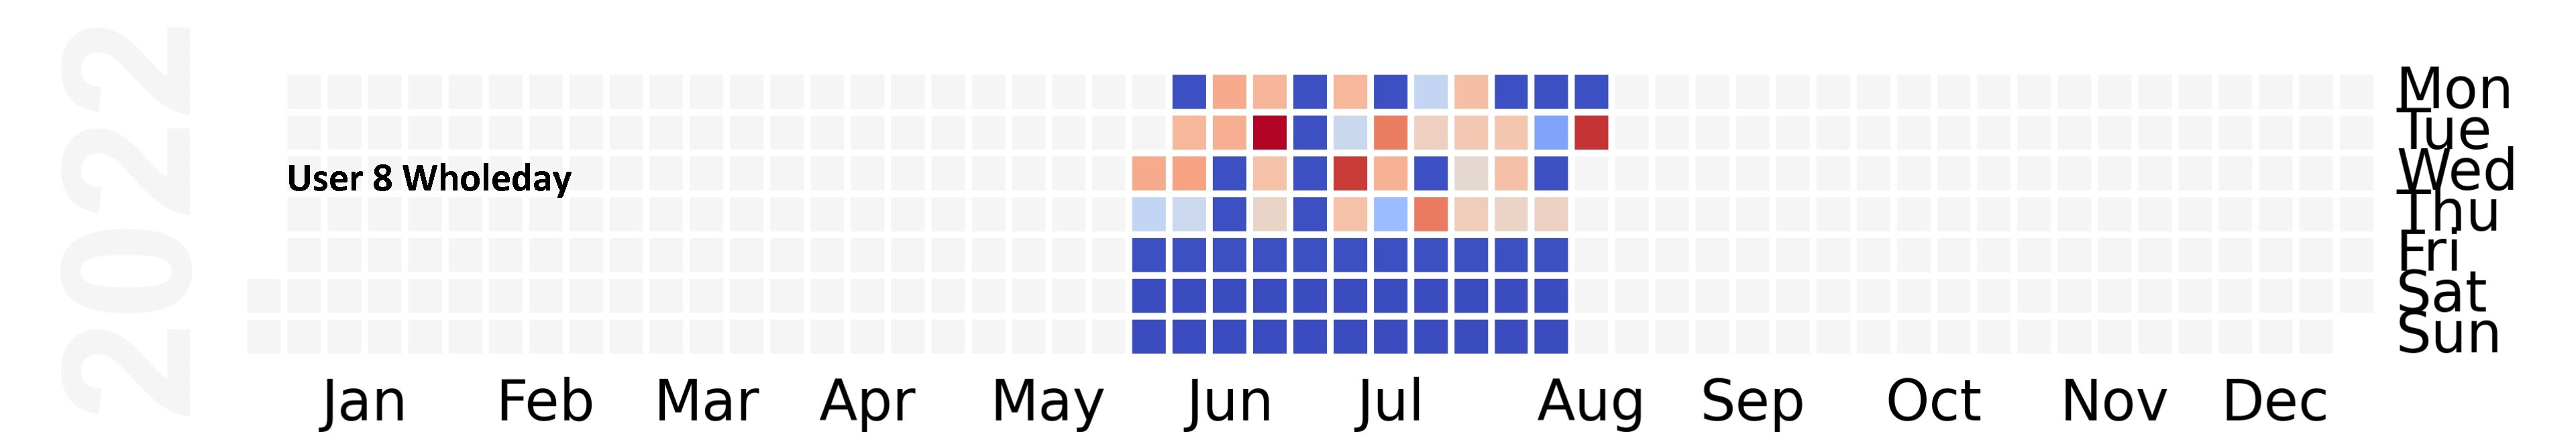
\includegraphics[width=0.5\textwidth]{images/heatmaps/user_8_wholeday_cal.png}}
    \subfloat{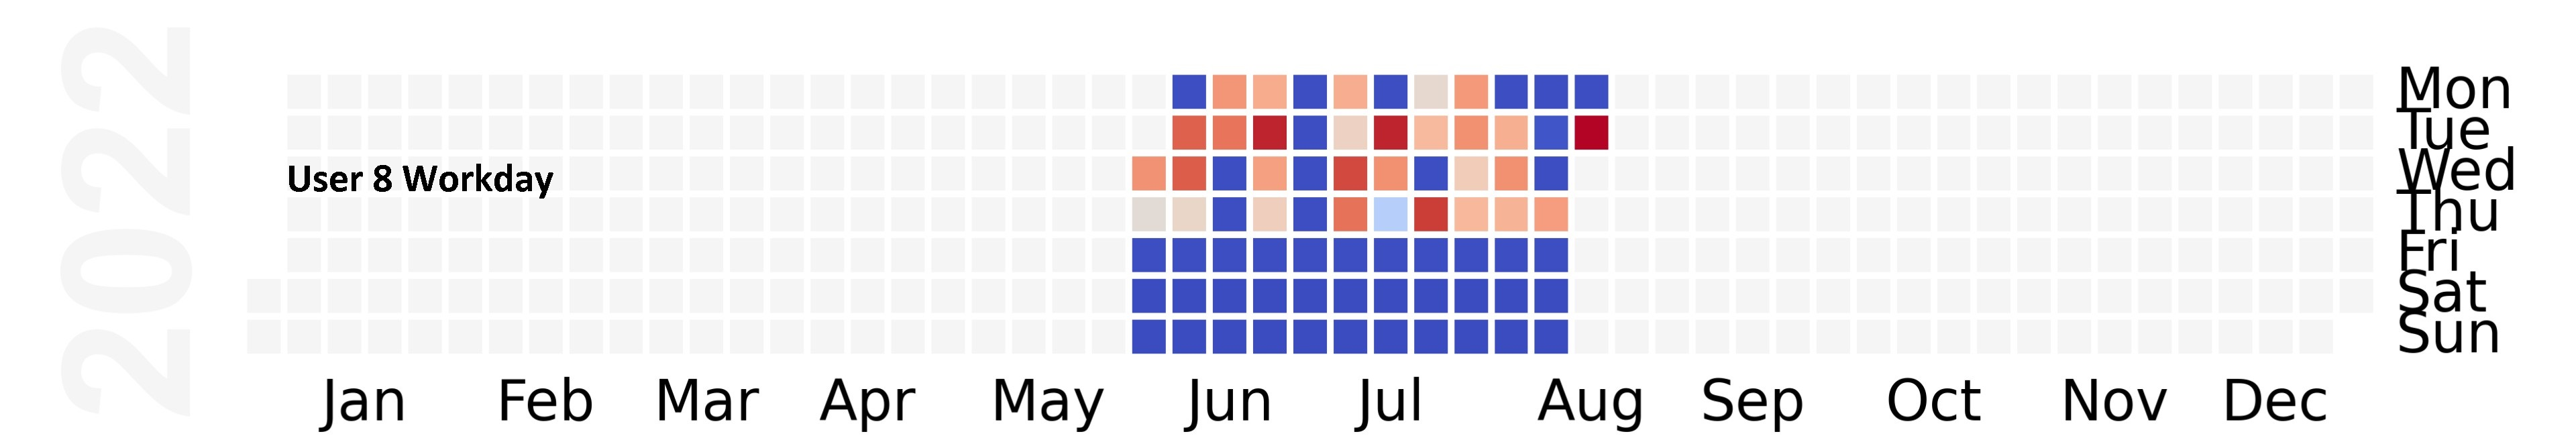
\includegraphics[width=0.5\textwidth]{images/heatmaps/user_8_workday_cal.png}}\newline
    \subfloat{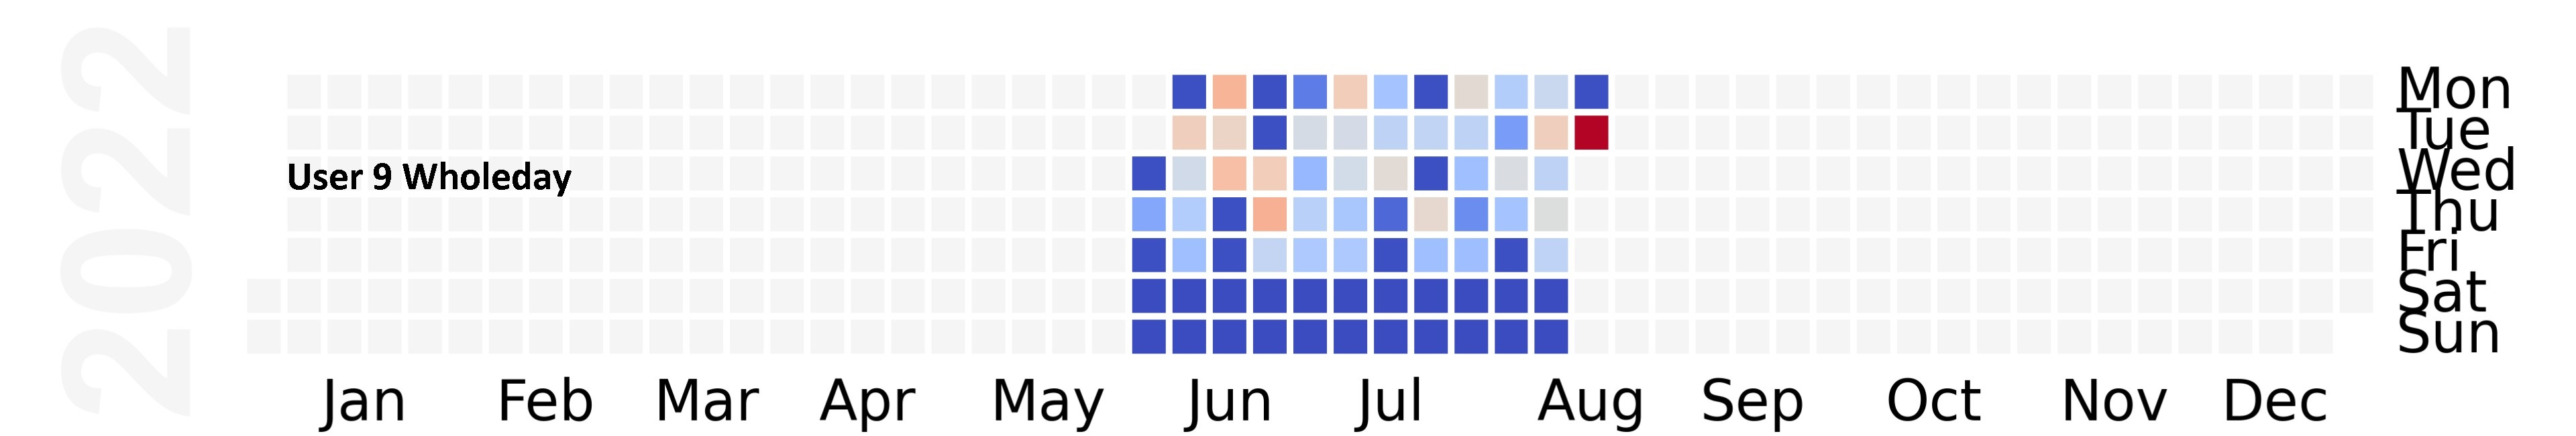
\includegraphics[width=0.5\textwidth]{images/heatmaps/user_9_wholeday_cal.png}}
    \subfloat{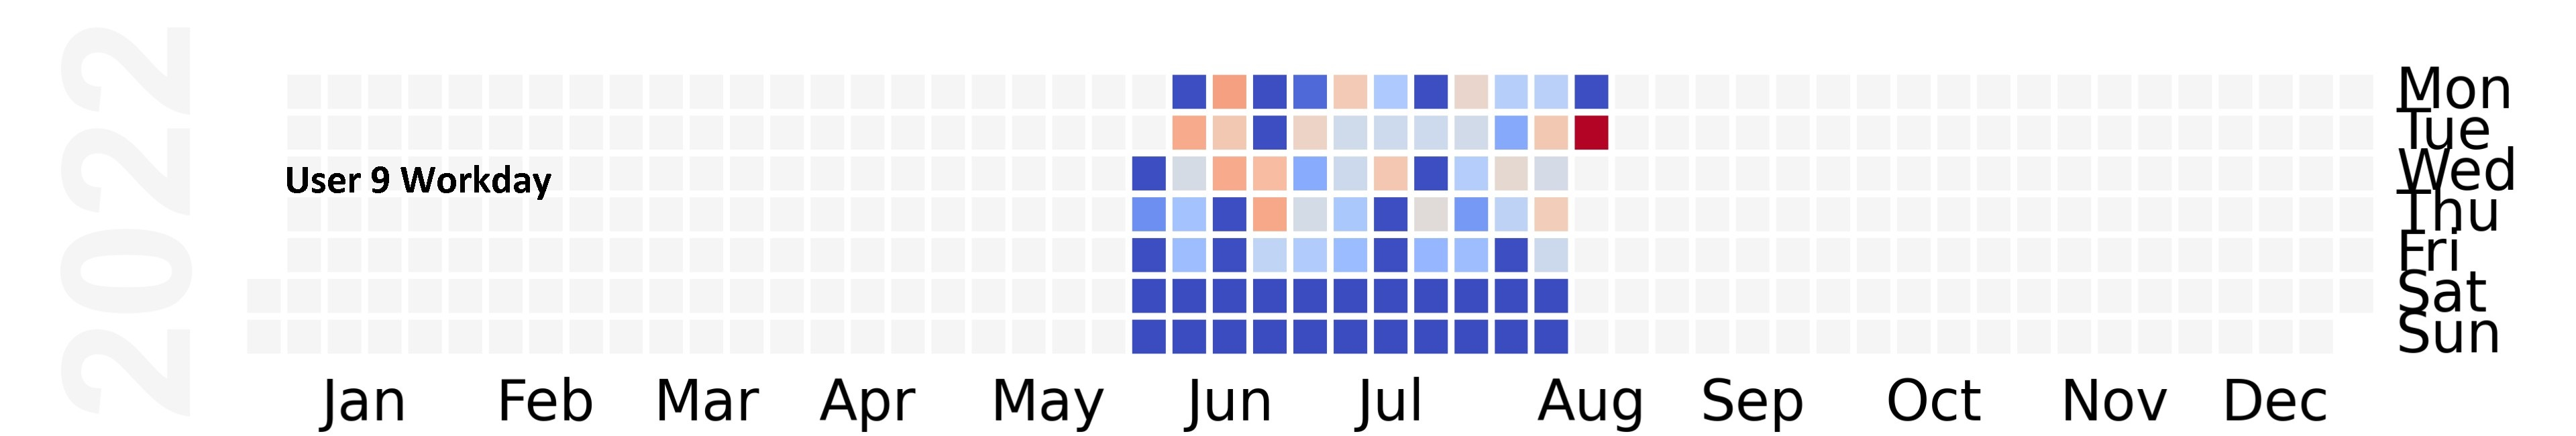
\includegraphics[width=0.5\textwidth]{images/heatmaps/user_9_workday_cal.png}}\newline
    \subfloat{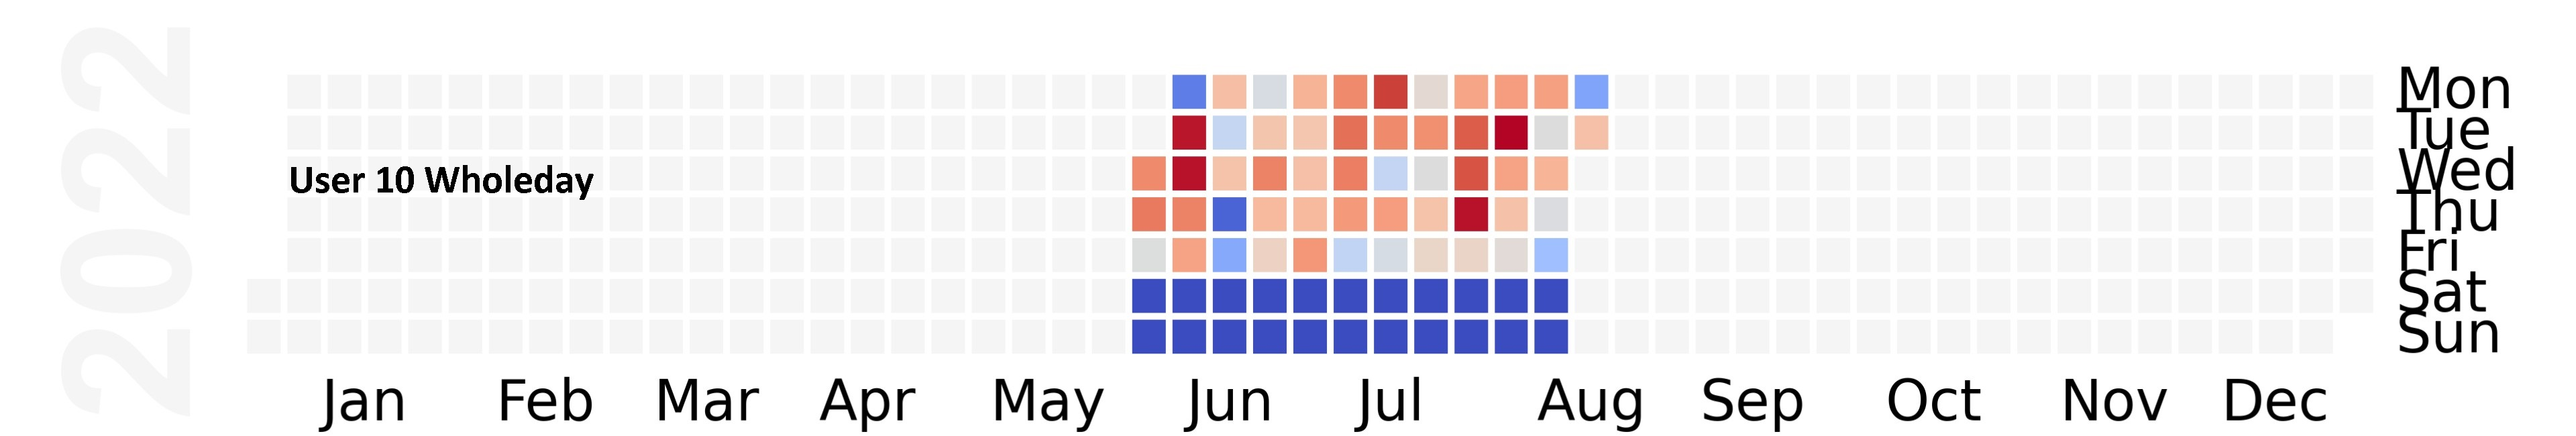
\includegraphics[width=0.5\textwidth]{images/heatmaps/user_10_wholeday_cal.png}}
    \subfloat{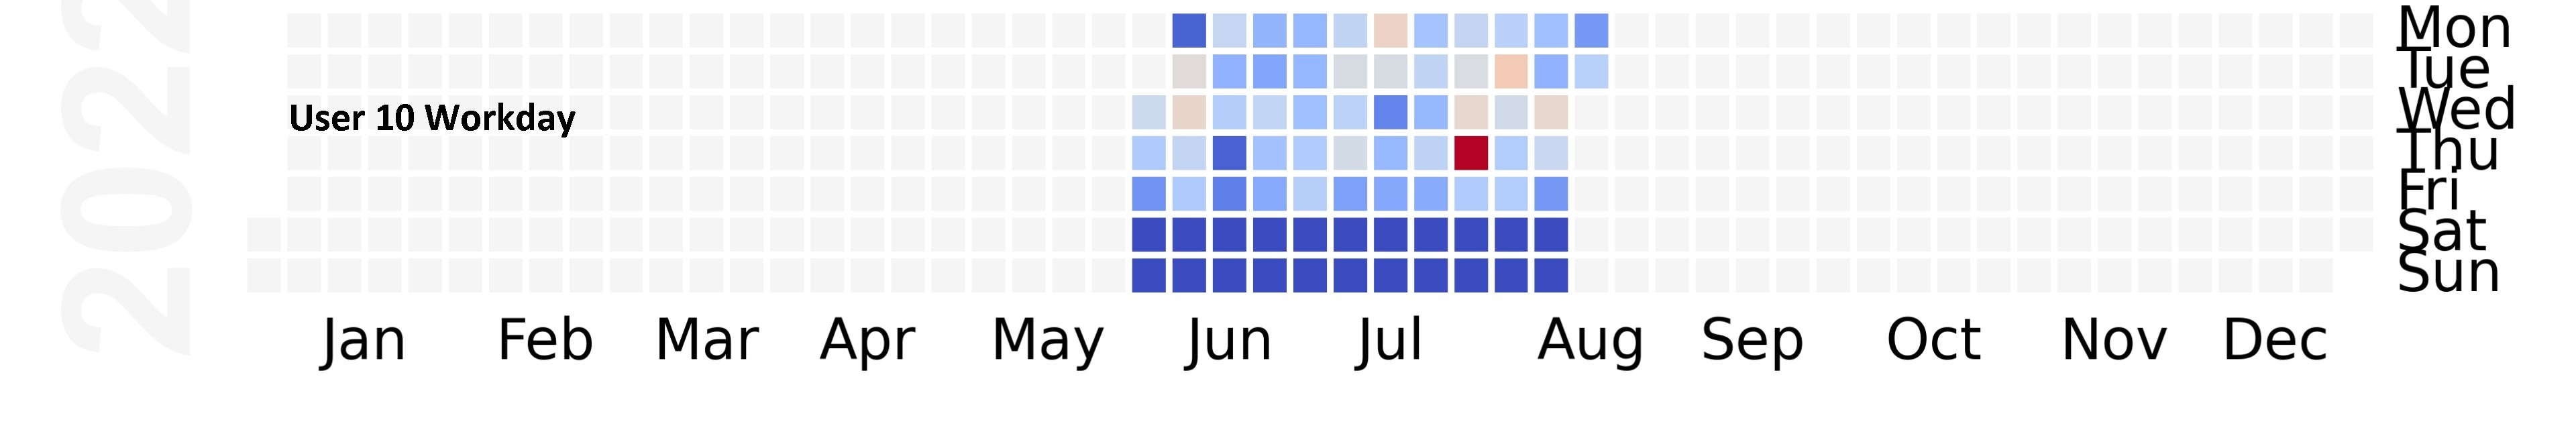
\includegraphics[width=0.5\textwidth]{images/heatmaps/user_10_workday_cal.png}}\newline
    \subfloat{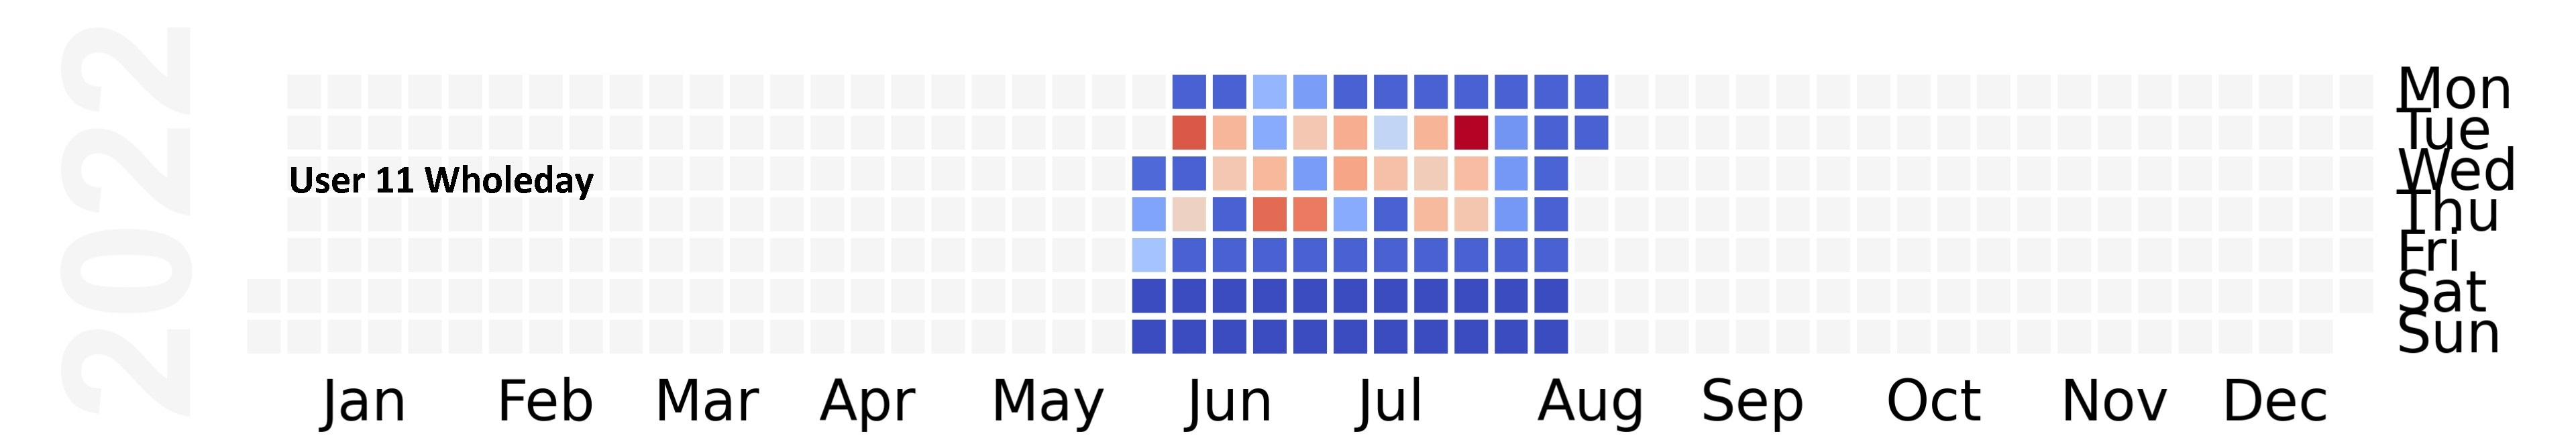
\includegraphics[width=0.5\textwidth]{images/heatmaps/user_11_wholeday_cal.png}}
    \subfloat{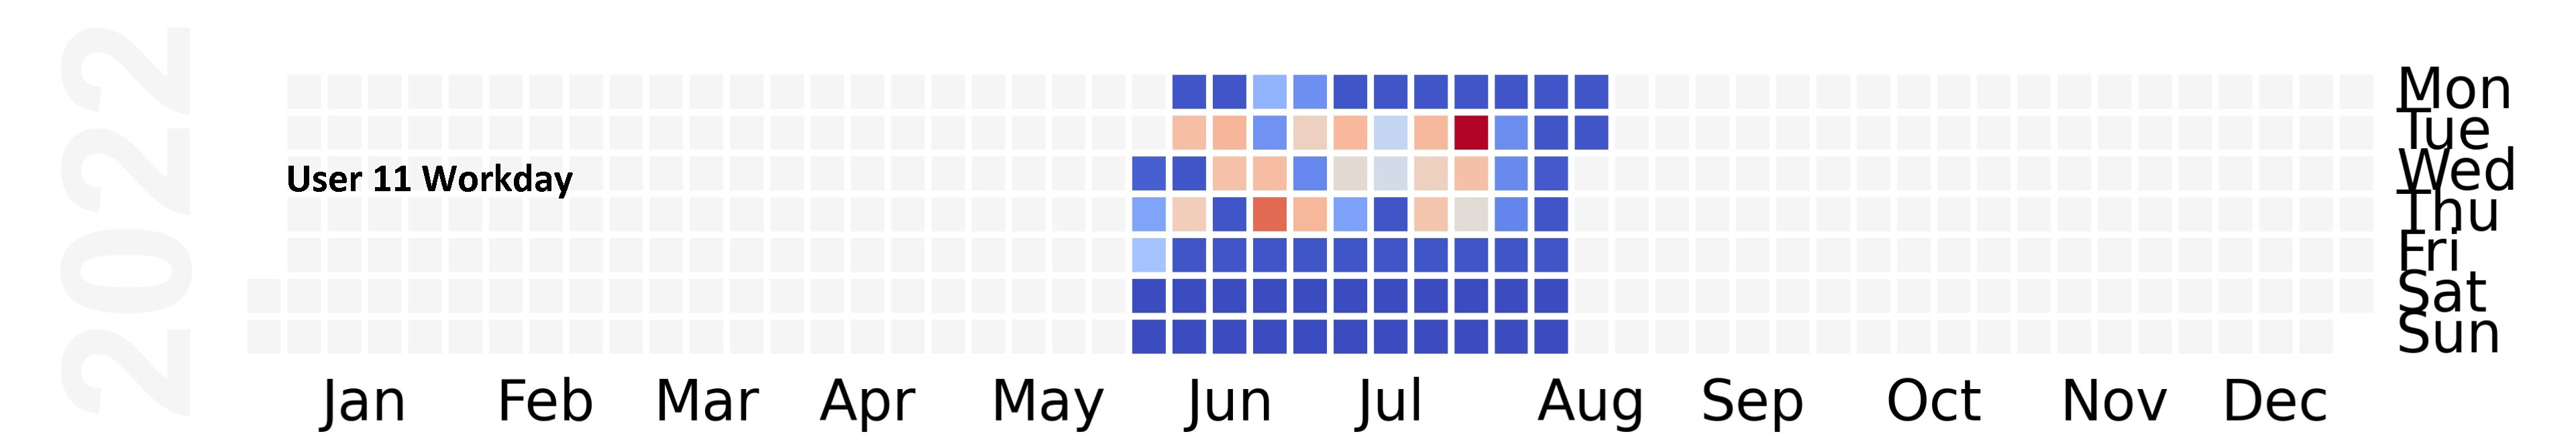
\includegraphics[width=0.5\textwidth]{images/heatmaps/user_11_workday_cal.png}}\newline
    \subfloat{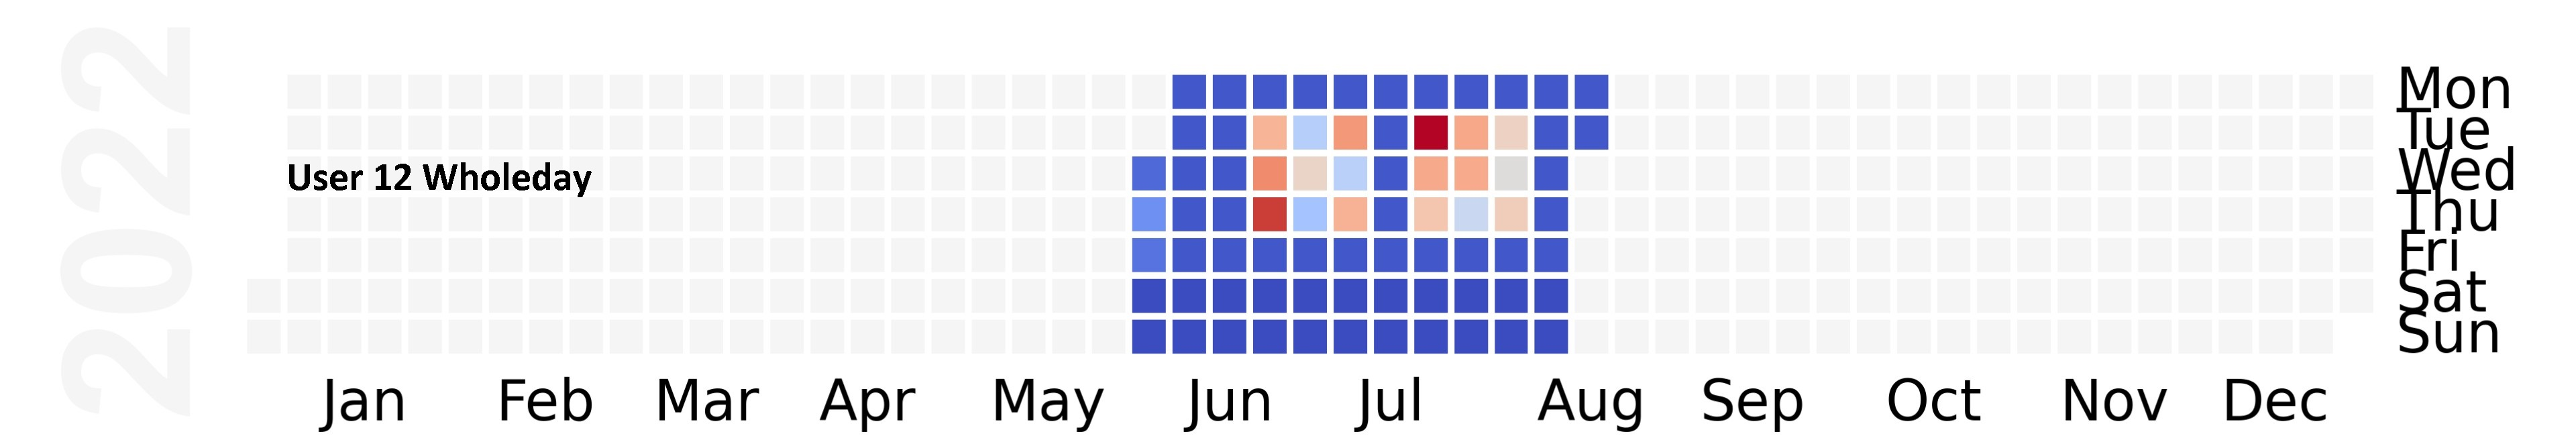
\includegraphics[width=0.5\textwidth]{images/heatmaps/user_12_wholeday_cal.png}}
    \subfloat{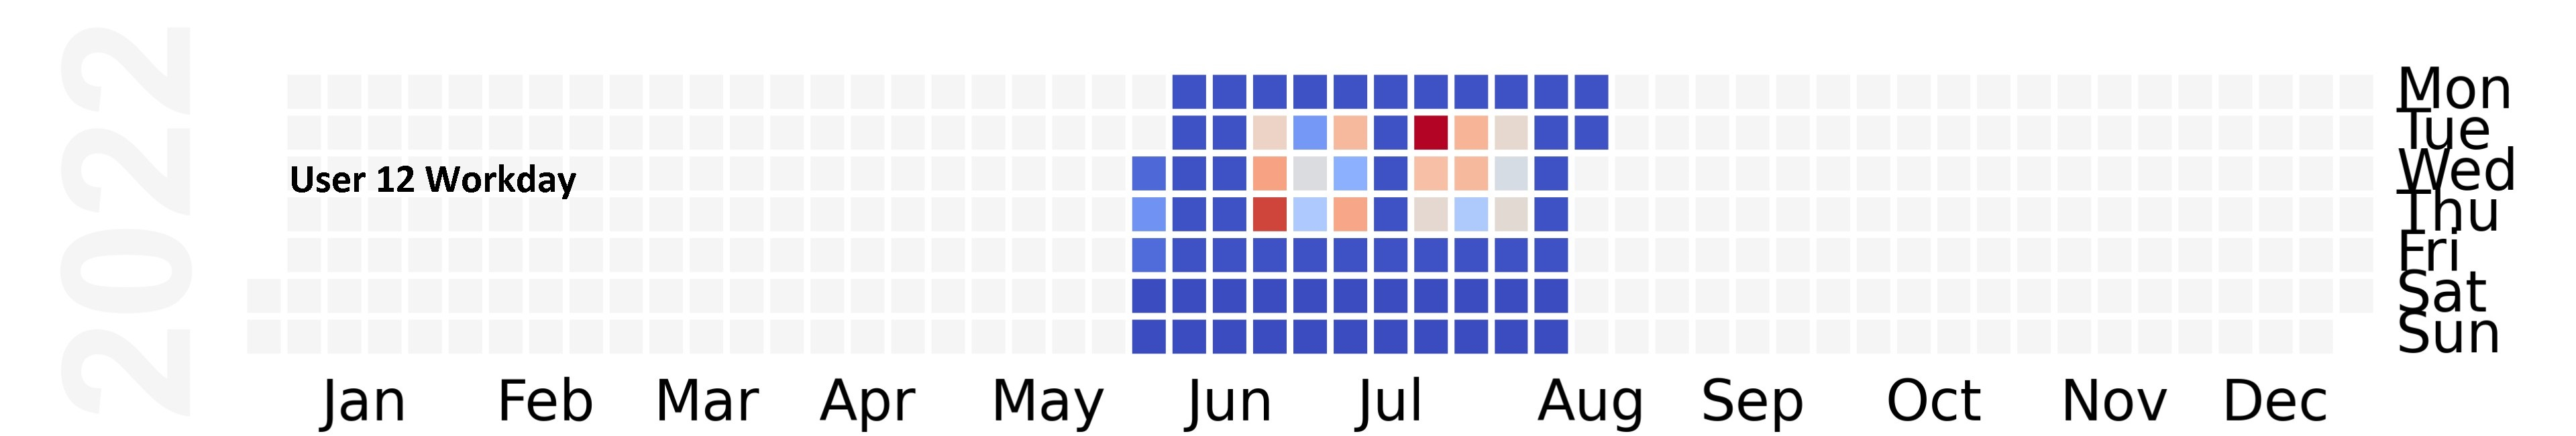
\includegraphics[width=0.5\textwidth]{images/heatmaps/user_12_workday_cal.png}}\newline
    \subfloat{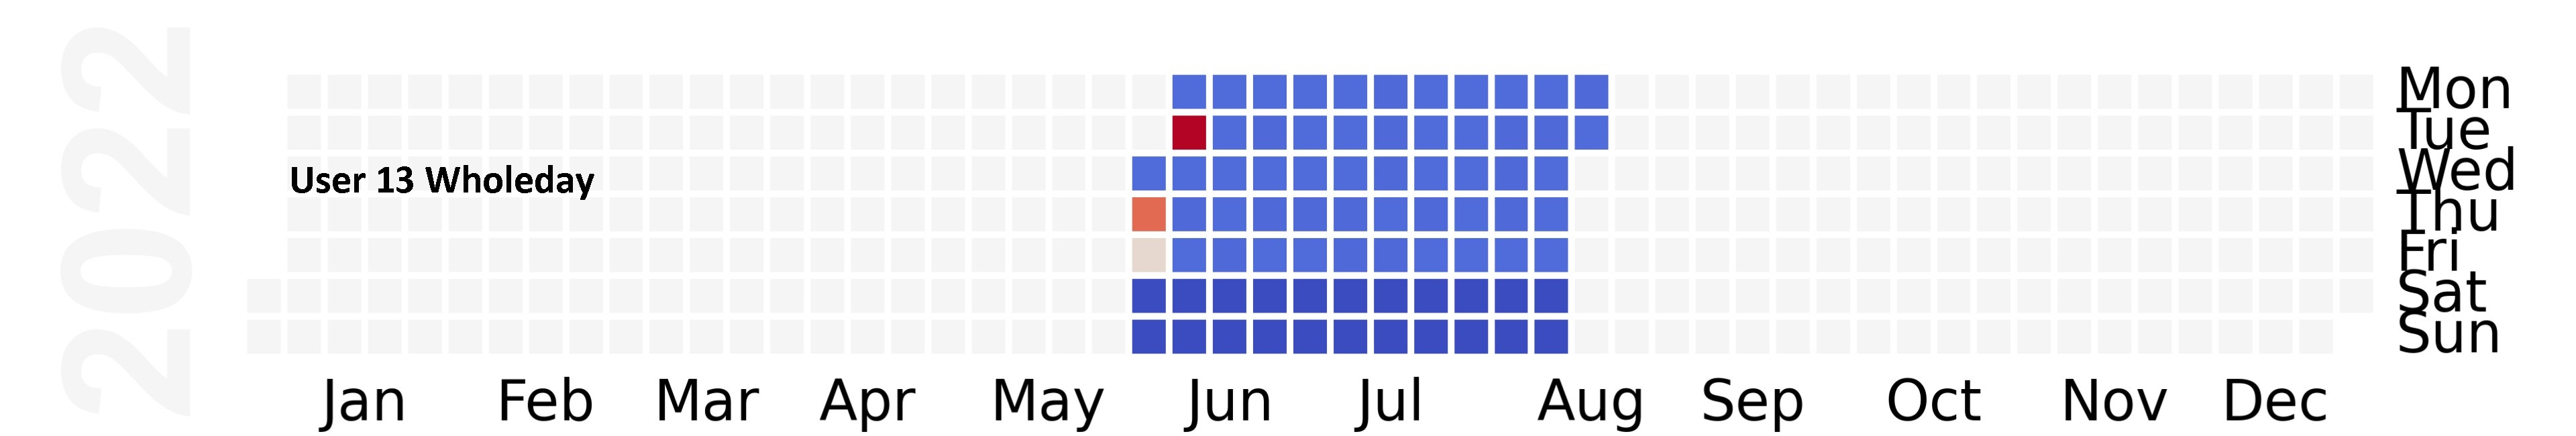
\includegraphics[width=0.5\textwidth]{images/heatmaps/user_13_wholeday_cal.png}}
    \subfloat{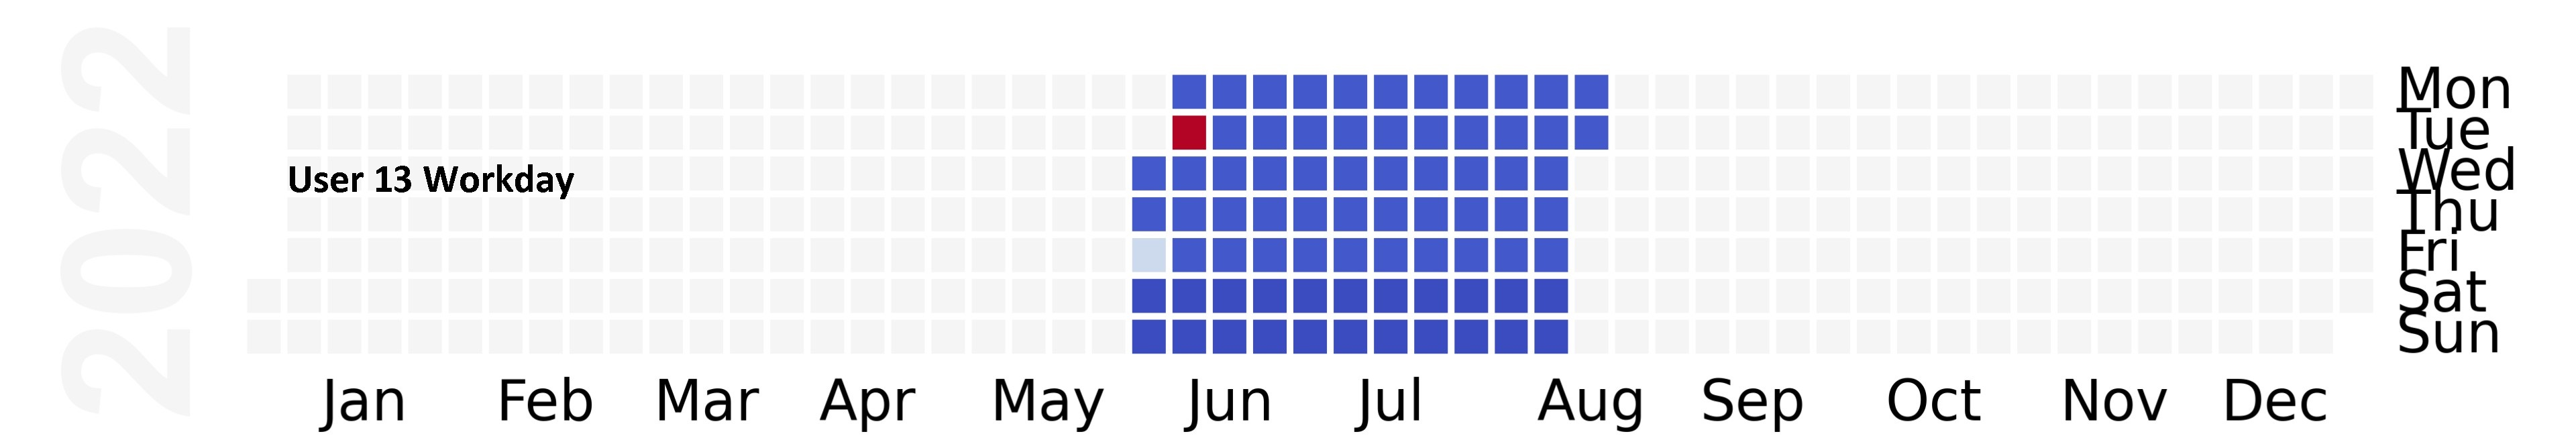
\includegraphics[width=0.5\textwidth]{images/heatmaps/user_13_workday_cal.png}}\newline
    \subfloat{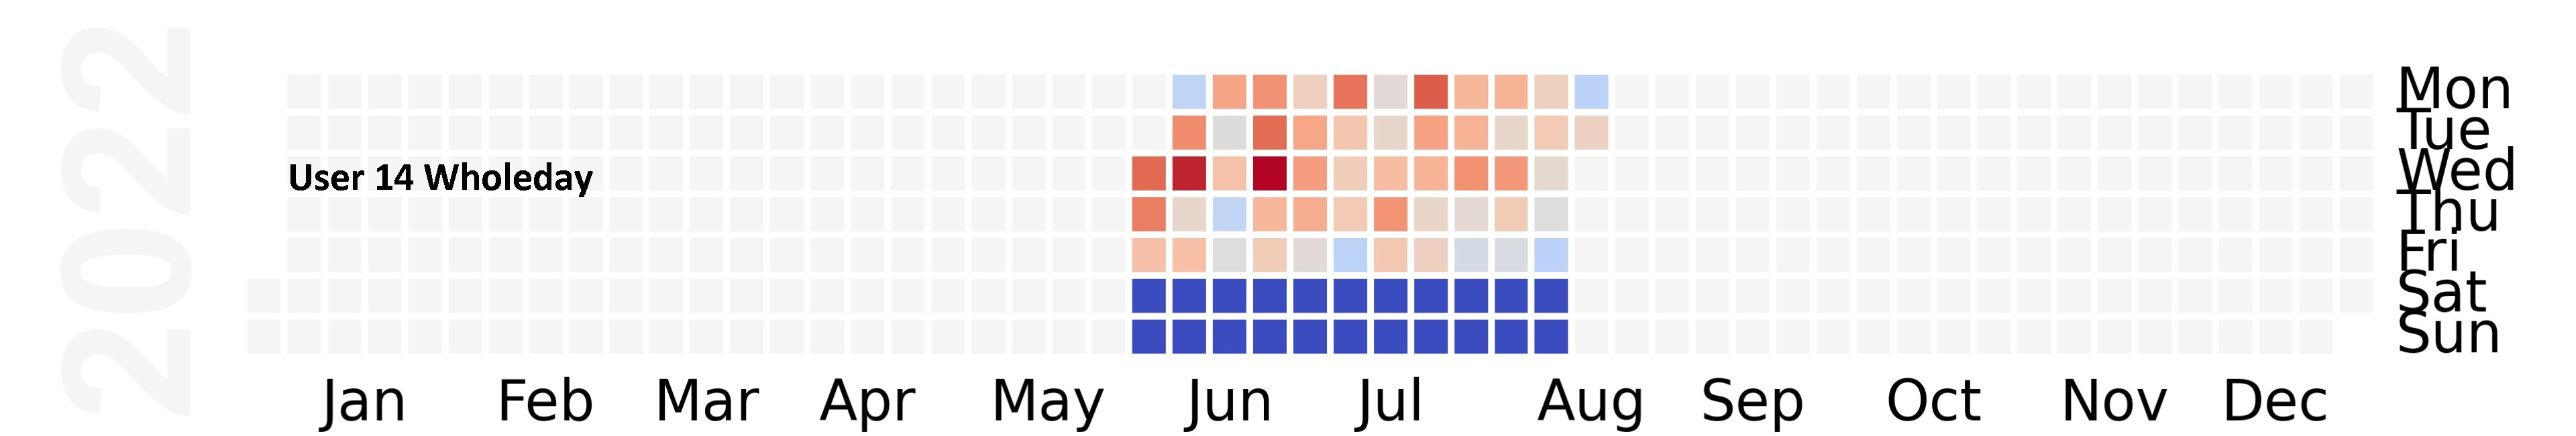
\includegraphics[width=0.5\textwidth]{images/heatmaps/user_14_wholeday_cal.png}}
    \subfloat{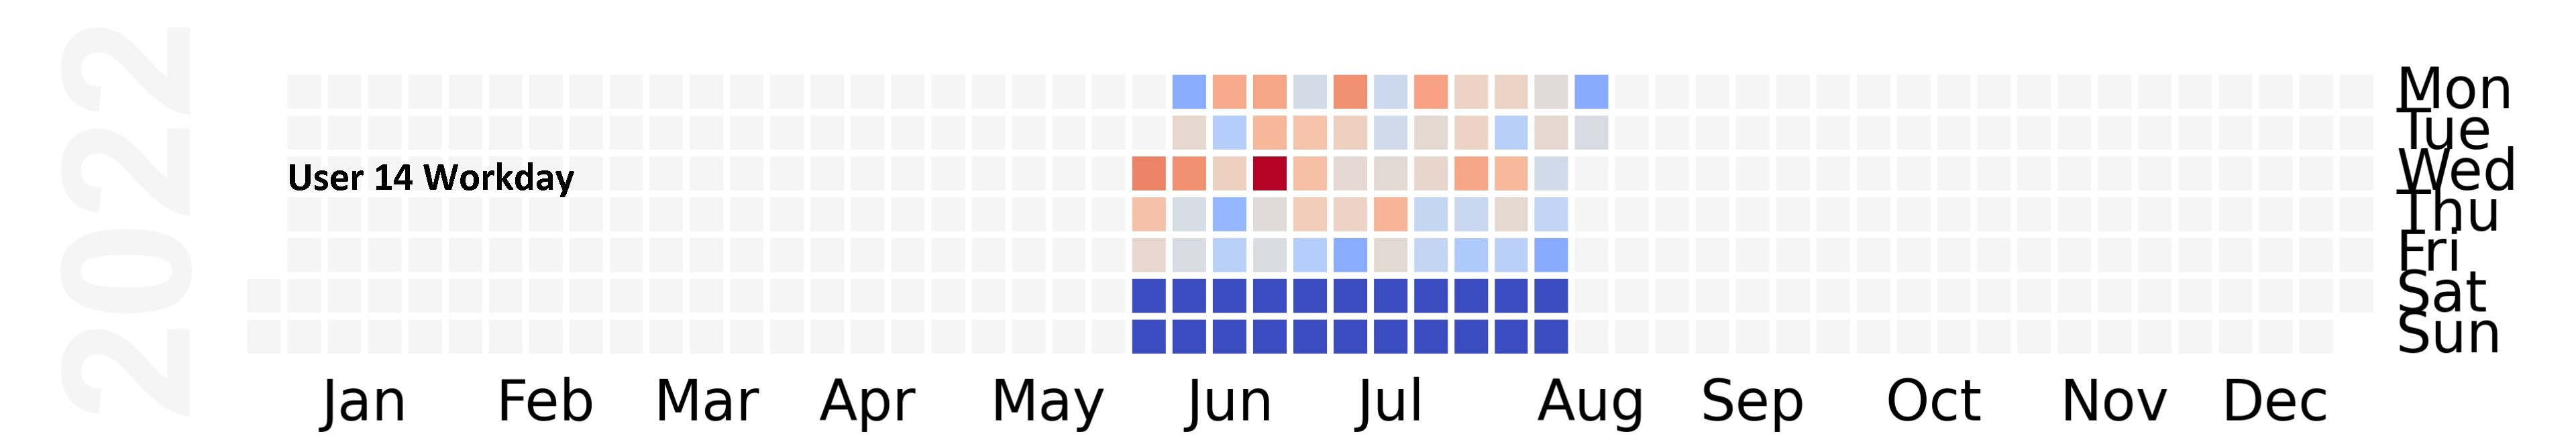
\includegraphics[width=0.5\textwidth]{images/heatmaps/user_14_workday_cal.png}}\newline
    \subfloat{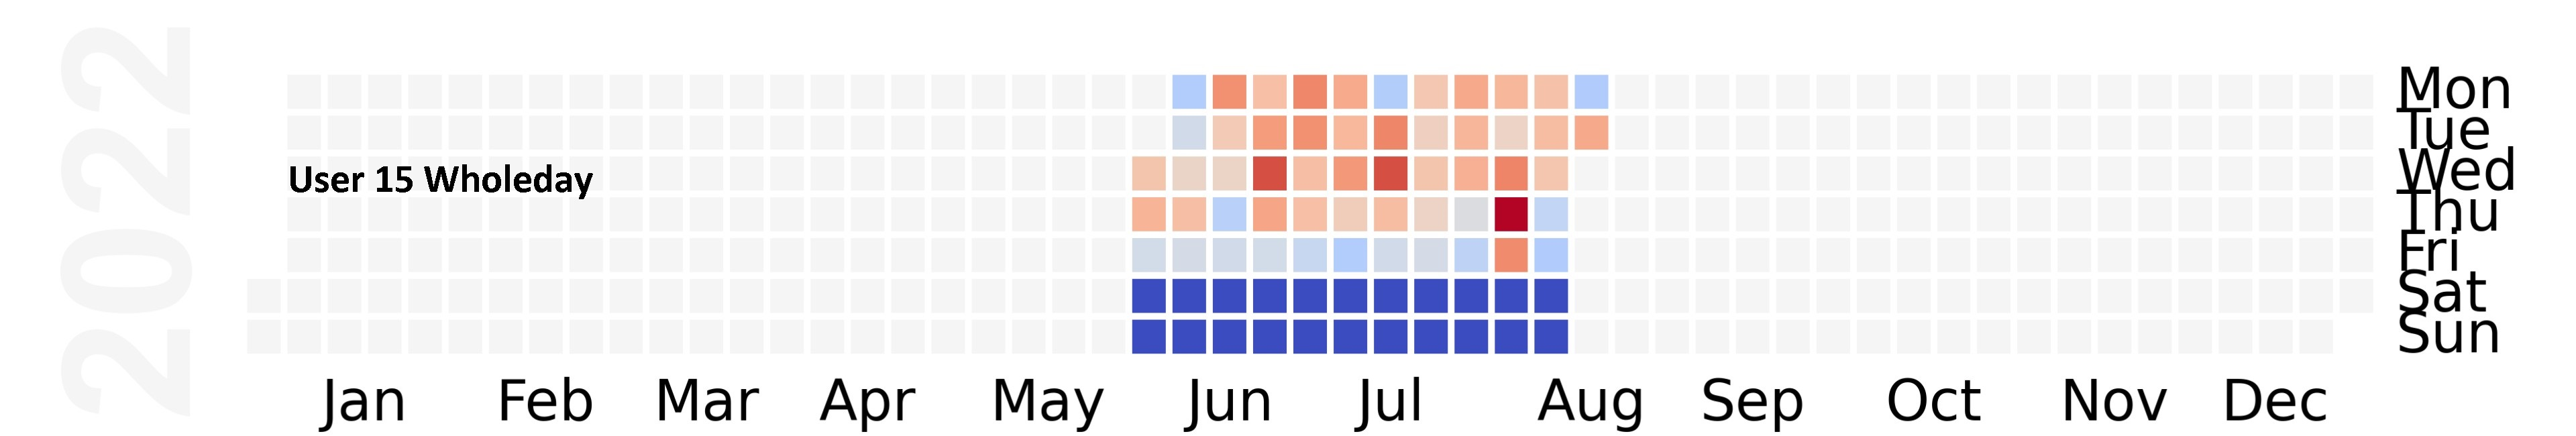
\includegraphics[width=0.5\textwidth]{images/heatmaps/user_15_wholeday_cal.png}}
    \subfloat{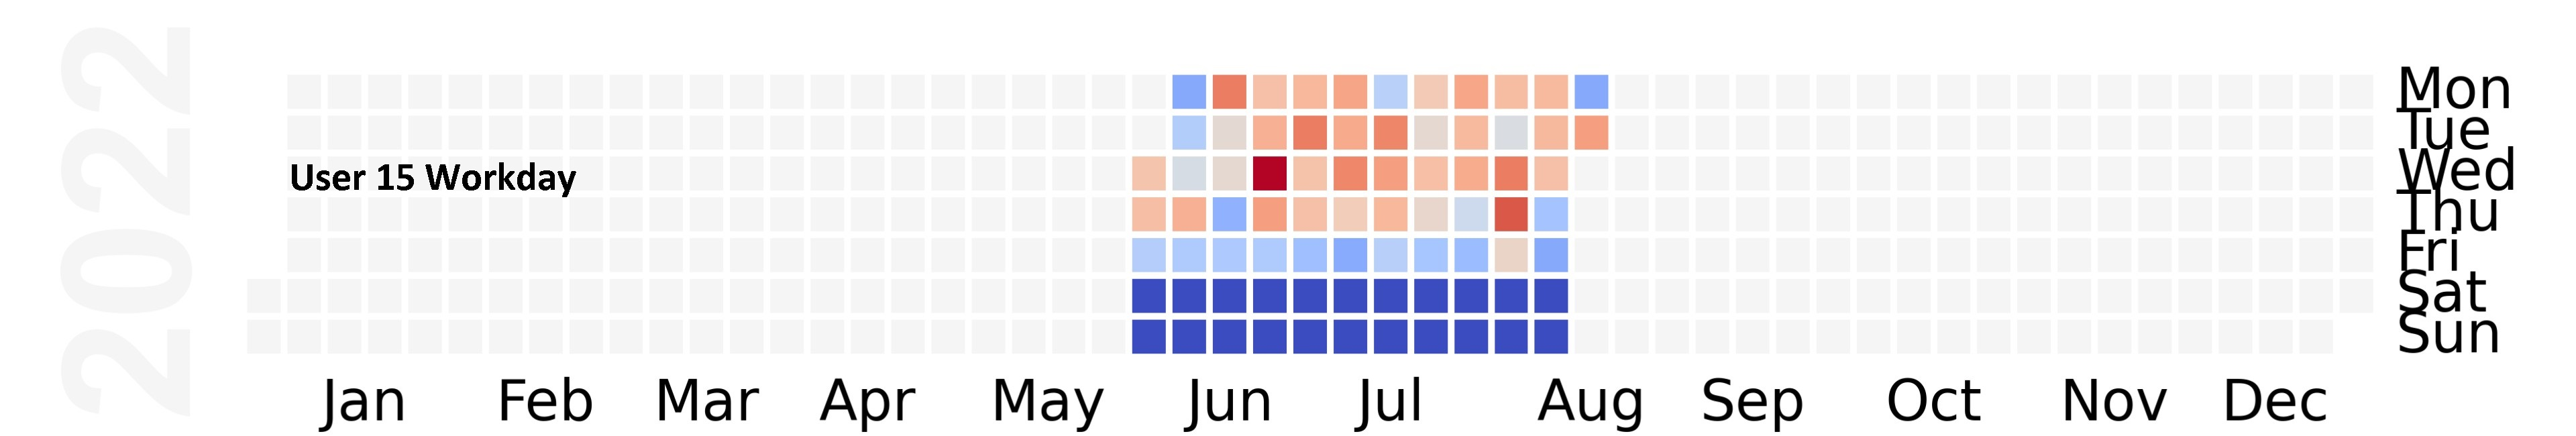
\includegraphics[width=0.5\textwidth]{images/heatmaps/user_15_workday_cal.png}}\newline
    \caption{\centering Comparison of the consumption of each user (Row 1-15) over time. Consumption is only considered without weekends with averages during the weekday (left) and working hours (right).}
    \label{fig:user_comparison}
\end{figure}
\noindent The observation of reduced consumption on Fridays is increasingly clear using the illustration in figure \ref{fig:office_consumption}. The increased attendance on Wednesday in calendar week 25, as well as Tuesday in the last week is clearly distinguishable. By comparing single user heat maps to the summation can show differentiation between quantitative consumption peaks (consumption due to a higher amount of people) and qualitative peaks (high spikes in consumption due to changes in the workload/ type of labor).
\begin{figure}[ht]
	\centering
	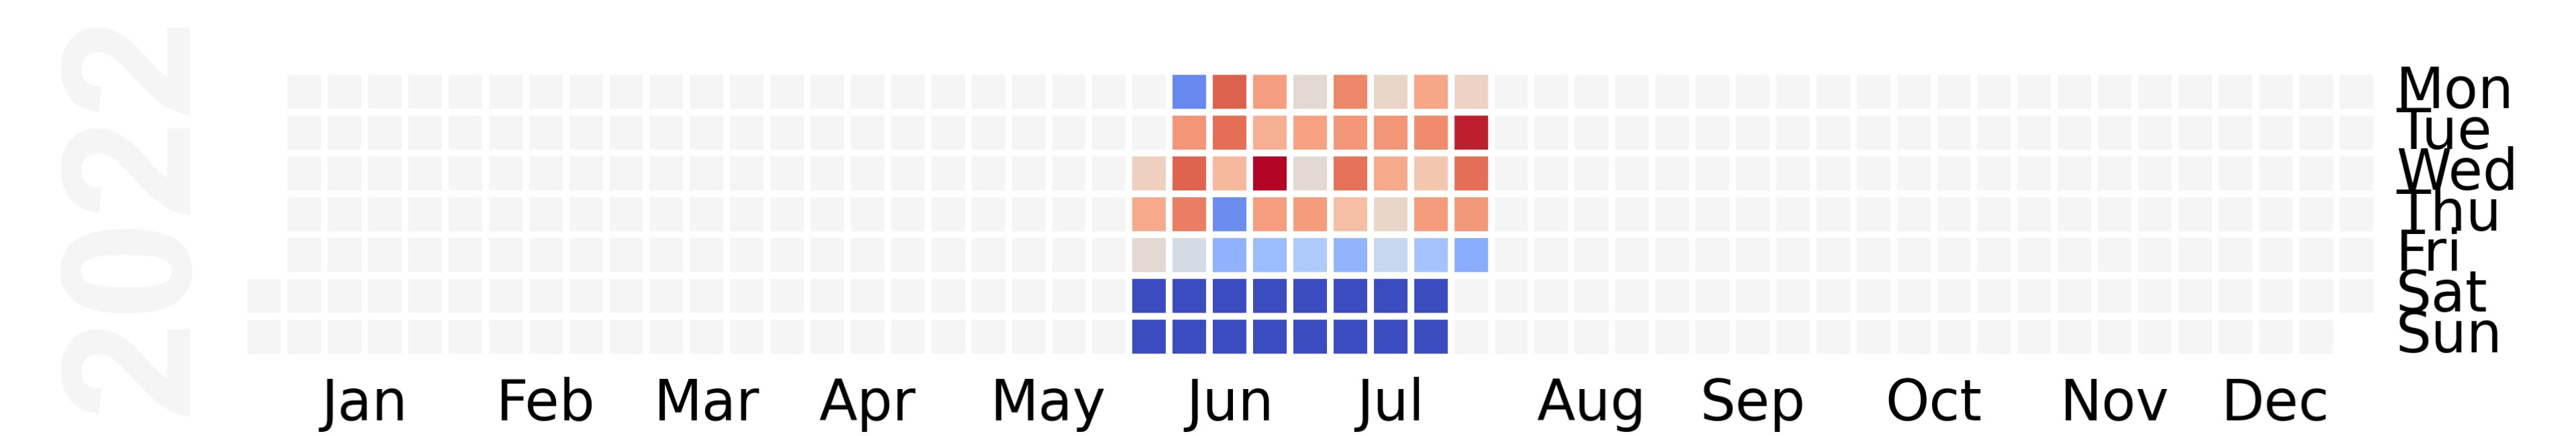
\includegraphics[width=\textwidth]{images/heatmaps/workday_cal.png}
	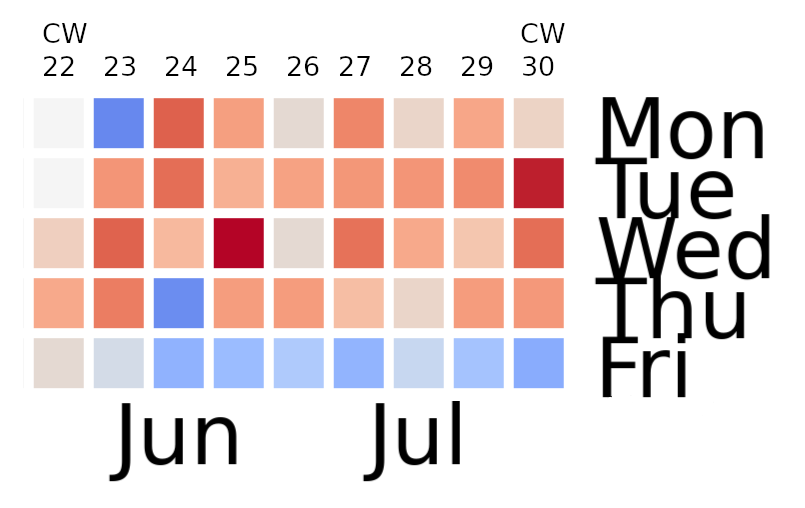
\includegraphics[width=\textwidth]{workday_cal_edit2.png}
	\caption{Heat map of the sum of all sensors during usual office hours (work hours on \glspl{workday}).Above the unedited plot, below an edited version to improve visibility.}
	\label{fig:office_consumption}
\end{figure}
\begin{figure}[ht]
	\centering
	Personal Computers
	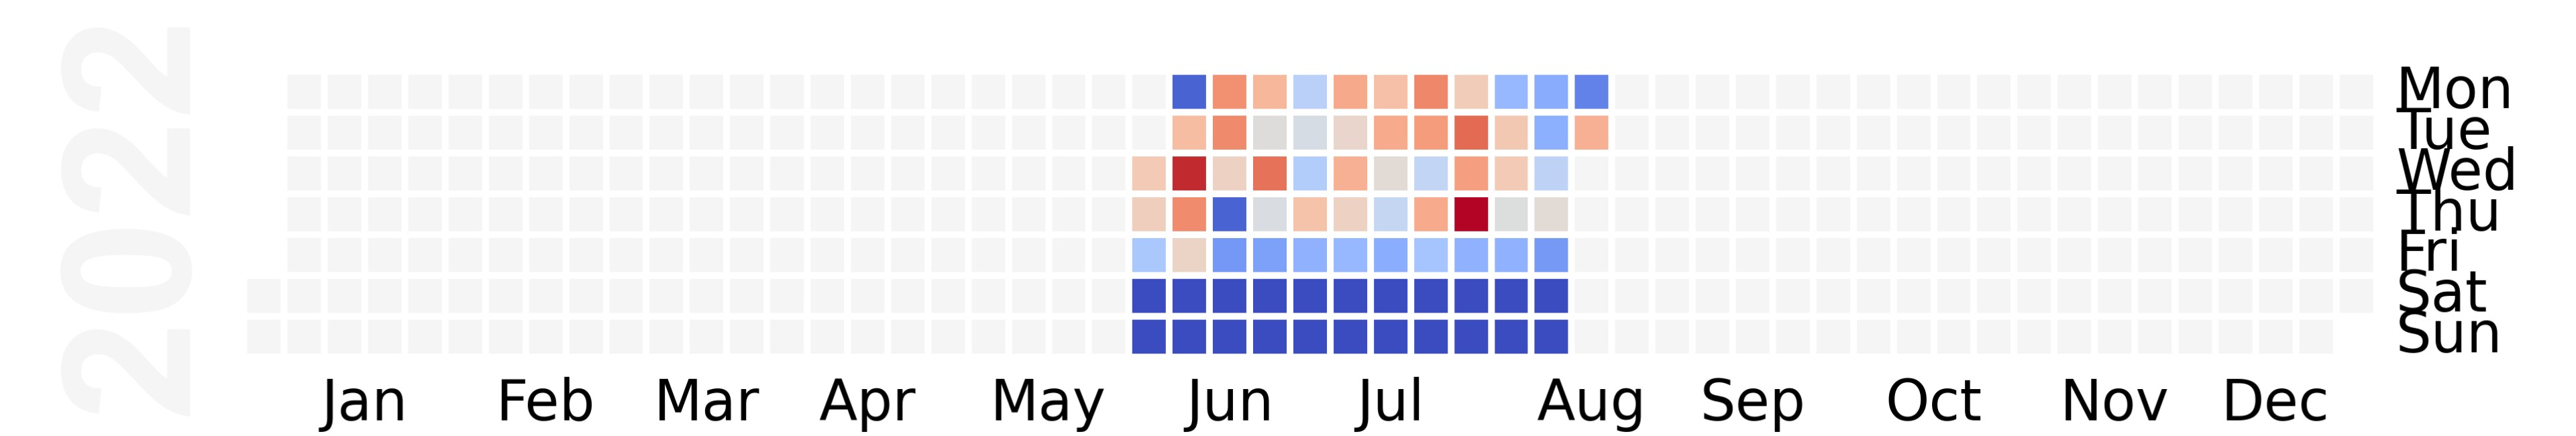
\includegraphics[width=\textwidth]{images/heatmaps/devicetype_PC_workday_cal.png}
	\caption{Heat map of the sum of all PC sensors during usual office hours (measured during \glspl{workday}).}
	\label{fig:pc_hm}
\end{figure}
\noindent As expected the consumption patterns of Monitors highly correlate the pattern given by PC measurements, which can be compared using figures \ref{fig:pc_hm} and \ref{fig:mon_hm}. In comparison the consumptions of utility devices and printer do not match nearly as neatly. In the case of printers the differentiation is harder due to the pronounced consumtpion spike on Wednesday of CW 27.
\begin{figure}[ht]
	\centering
	Monitors
	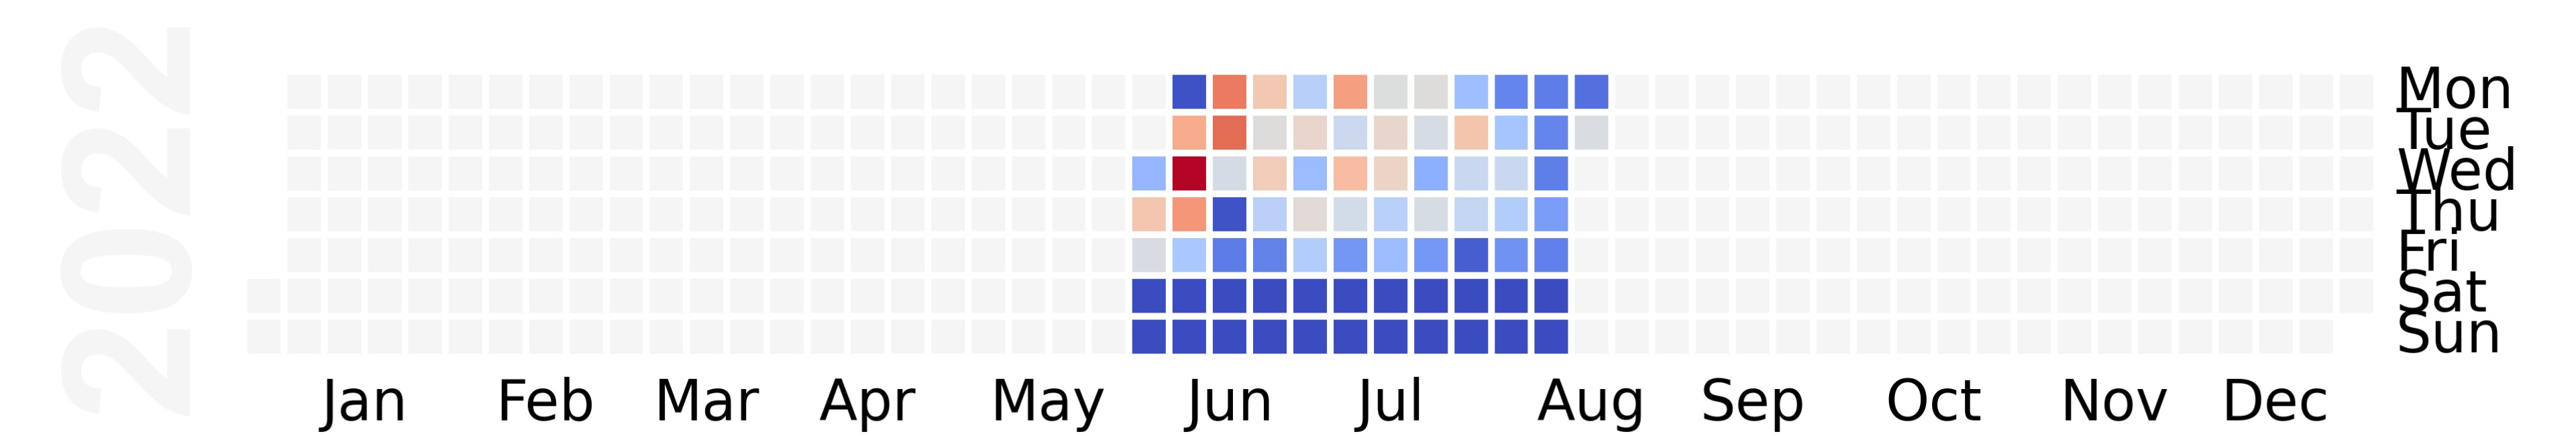
\includegraphics[width=\textwidth]{images/heatmaps/devicetype_Monitor_workday_cal.png}
	\caption{Heat map of the sum of all monitor sensors during usual office hours (measured during \glspl{workday}).}
	\label{fig:mon_hm}
\end{figure}
\begin{figure}[ht]
	\centering
	Printer
	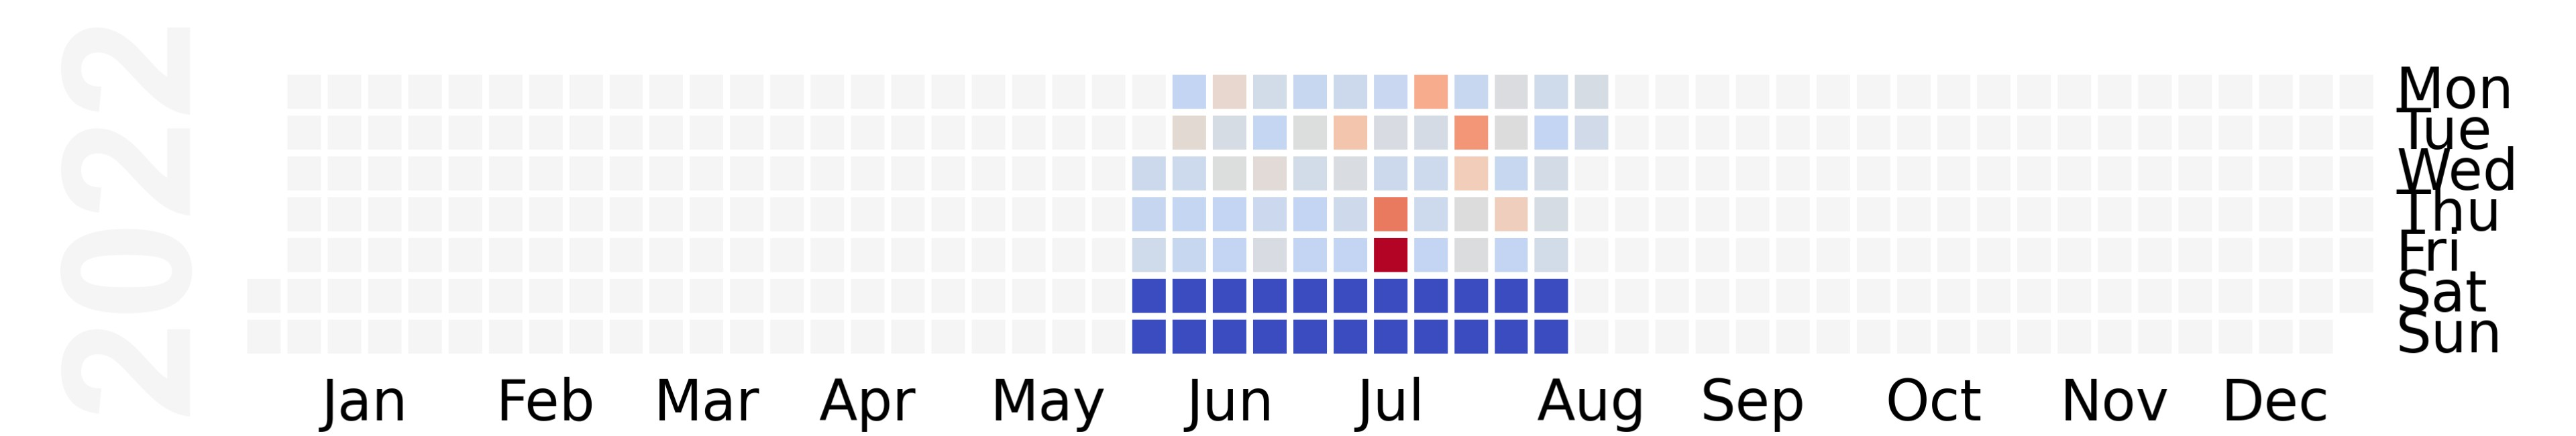
\includegraphics[width=\textwidth]{images/heatmaps/devicetype_Printer_workday_cal.png}
	\caption{Heat map of the sum of all printer sensors during usual office hours (measured during \glspl{workday}).}
	\label{fig:printer_hm}
\end{figure}

\begin{figure}[ht]
	\centering
	Utilities	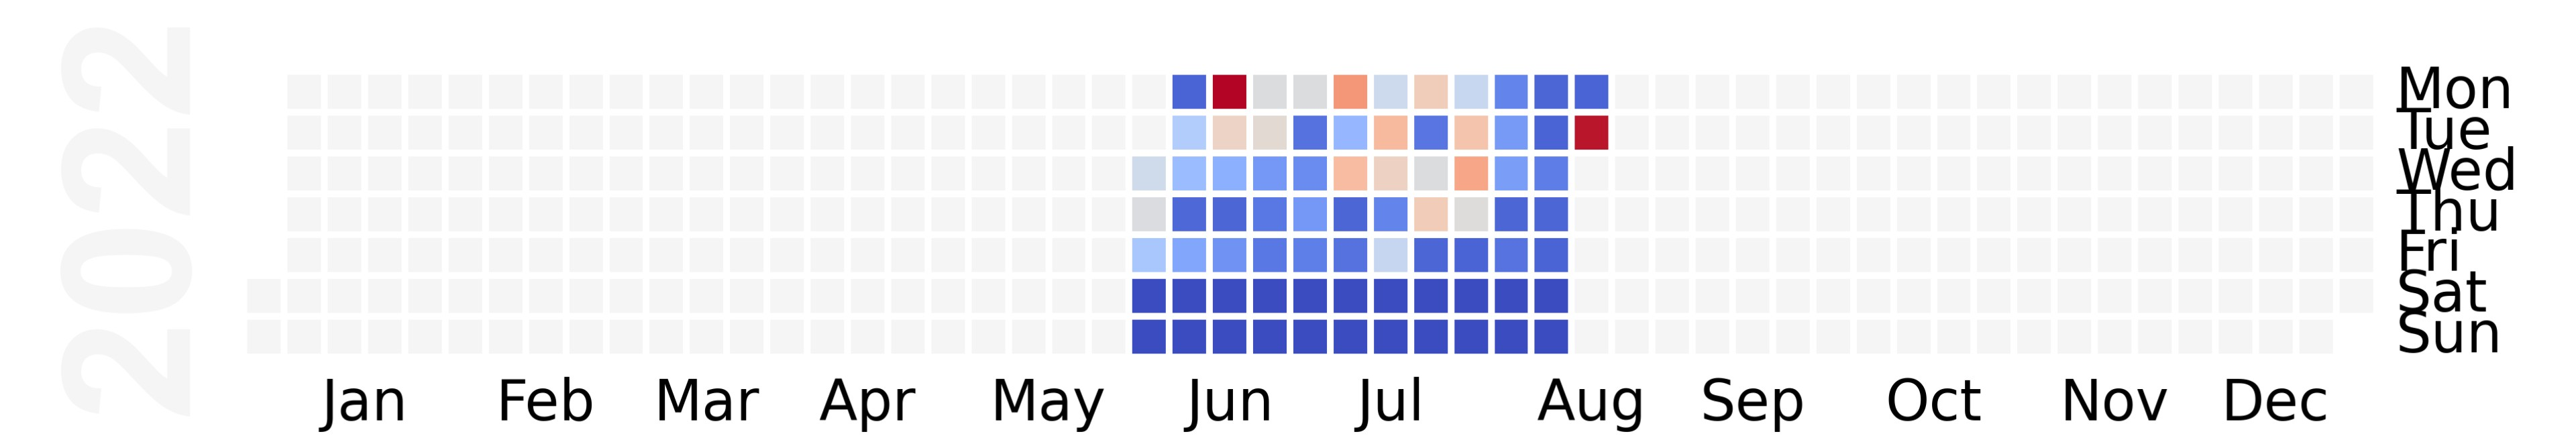
\includegraphics[width=\textwidth]{images/heatmaps/devicetype_Utility_workday_cal.png}
	\caption{Heat map of the sum of all utility sensors during usual office hours (measured during \glspl{workday}).}
	\label{fig:util_hm}
\end{figure}

\subsubsection{\acrfull{rpmt}}\label{subsec:RPMT}
To allow an even more interactive approach to data exploration, the Grafana service as described in the section \ref{subsec:software} allows creation of interactive dashboards. As an example application, in this work a sample dashboard that aims to be used as a motivational tool can be examined. A full screenshot of the dashboard can be seen in figure \ref{fig:dashboard}.\\
Besides showing overview data, Grafana can be used to send notifications if certain thresholds are crossed, for example by using telegram or discord bots. Address to access the Grafana service is shown in table \ref{tab:access} located of section \ref{subsec:hardware}.
\begin{figure}[h]
	\centering	
	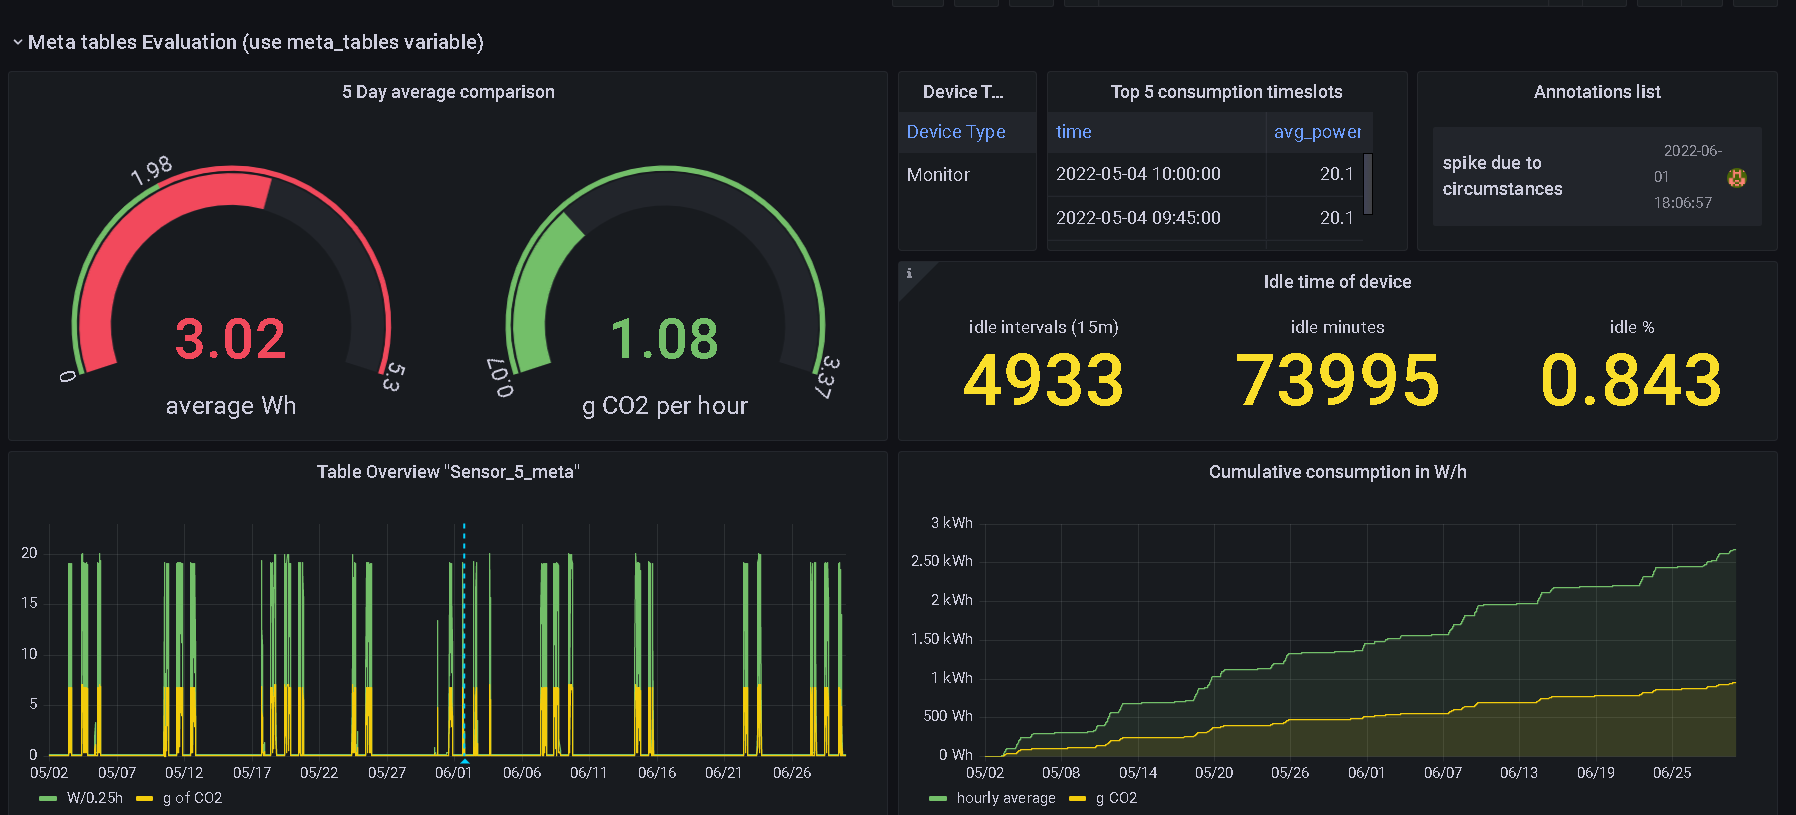
\includegraphics[width=\textwidth]{images/RPMT.png}
	\caption{Screenshot of the \acrshort{rpmt} dashboard. From top left to bottom right there are panels showing 5 day comparisons to similar devices, the device type, an overview of annotations, the overview of elapsed idle time of the device. the power consumption as a time series, and the cumulative time series with the respective estimated CO$_2$ footprint.}
	\label{fig:dashboard}
\end{figure}